% Hamad Medical Corporation
% Georges Younes

\section{Clinical Validation and Assessment}\label{sec:clinical_validation}

\begin{itemize}
  \item RARP Surgical substep PR 1 \path{Document4_RARP_Surgical_Substeps.pdf}
  \item Suturing alignment diagrams PR 2 \path{anastomosis.pdf}
  \item Extract suturing alignment diagrams from aim 6 \path{2012.hsmr.docx.pdf}
\end{itemize}

\hrule%

\subsection{Validation and Assessment}\label{ssec:validation_assessment}

% \textbf{\textcolor{red}{Add definitions of validities and summative/predictive, \etc. }}

Validation is an iterative assessment process throughout the prototype's development cycle to evaluate it from different perspectives: how it looks, how efficient it is, \etc. We choose to conduct face, content and construct validity to evaluate the simulator's realism, appropriateness as a teaching modality and how good it is to differentiate between novice and expert surgeons, respectively.
Face validity refers to the test conducted to assess the subjective realism of the simulator by different urologists that have expertise in robot-assisted radical prostatectomy (RARP). Content validity refers to test is conducted to assess the simulator’s appropriateness as a teaching modality. Construct validity refers to the test that measures how good is the simulator to differentiate between different skills,by collecting various parameters and checking the difference between them when it comes to novice or expert surgeon, for example.
We have developed a validation protocol to be performed after one or few set of features upon the release of a new prototype version. Features shall be assessed by a set of urologists to incorporate their feedback in the next prototype version.

Before the implementation starts, meetings were held with urologists to explain the exact clinical steps, know the parameters to be evaluated by the simulator and how to quantify subjects' performance.

The following points came up during the initial discussion with the surgeons for validation and assessment of a surgical simulator:

\subsubsection{Face Validity}\label{sssec:face_validity}
\begin{itemize}
  \item Is Face validity dependent on hardware interface irrespective of the software simulation? If yes, as we will be using Mimic frame or Mantis Duo for interface, will the face validity be same as the studies published previously?
  \item Will the result be biased if the clinician providing input during the development phase is also included in evaluation?
  \item Some suggested sample subjective questionnaire to be recorded on Likert scale:
  \begin{itemize}
    \item The interface (hand-foot controllers/visualization interface) provided on the simulator is effective for working in the simulated environment?
    \item The device is sufficient accurate representation of the real robotic system?
  \end{itemize}
\end{itemize}


\subsubsection{Content Validity}\label{sssec:content_validity}
\begin{itemize}
  \item The subjective study will give a single value for content validity questions. Would it be sufficient?
  \item Will the result be biased if the clinician providing input during the development phase is also included in evaluation?
  \item Sample Subjective Questionnaire to be recorded on likert scale
  \begin{itemize}
    \item The 3D graphical exercises in the simulator are effective for teaching robotic skills
    \item The scoring system effectively communicates my performance on the exercise
    \item The scoring system effectively guides me to improve performance on the simulator
  \end{itemize}
\end{itemize}

\subsubsection{Construct Validity}\label{sssec:construct_validity}
\begin{itemize}
  \item Some sample objective data metric to be measured by system's software itself:
  \begin{itemize}
    \item Overall score (points) \eg resulting composite metric (total point score or percentage). Robotic surgeons set a relative value of each measure used in the composite score and depends upon the training need. The resulting composite score places the person in threshold levels (which is again defined by robotic surgeon) to evaluate the outcome of pass/fail/warning.
    \item Number of errors (count) \eg tissue ruptures or suture breaks, number of instrument collision, number of times object is grasped and dropped.
    \item Time to complete (seconds)
    \item Economy of motion (centimeters) \eg quality of resection, location and quality of placed sutures, blood loss, instrument going out of view, tissue damage cause by excessive instrument force or unwanted touching, optimum movement of camera.
  \end{itemize}
\end{itemize}




\hrule%

\subsection{Clinical Steps}\label{ssec:clinical}
The surgical sub-step of cutting the urethra during \acr{rarp} procedure was selected for generation of simulation scenario. The required surgical-steps during \acr{rarp} procedure includes:
\begin{enumerate*}[\em i\em)]
  \item Dropping the bladder,
  \item dividing the neck of the bladder,
  \item exposing the posterior lateral,
  \item cutting the urethra, and
  \item anastomosis.
\end{enumerate*}

Although the approach in performing the surgery might vary between surgeons, \eg whether they perform a transperitonial or an extraperitonial approach, in this project, we simulate only cutting the urethra, which is constant across different variations in terms of requirements, tools and approach.

Urethra dissection is performed by cutting the urethra close to the apex of the prostate, typically with cold scissors to avoid damaging the nearby nerves and structures. Before urethra cutting, cold cutting scissors are used to dissect around it. Occasionally, the \acr{ppl} is cauterized to block bleeding at the side, otherwise cautery is minimized as much as possible in this process as the monopolar current can spread to almost \SIrange{5}{7}{\milli\metre}, which might damage the nearby nerve bundles. The challenge in arriving at the site of the urethra cutting is in carefully dissecting around it. Around the urethra, there is a large vascular complex (called the Dorsal Venous Complex or Santorini's Plexus) and the \acr{ppl}, which the surgeon carefully approaches. As the surgeon dissects through this area, he will be able to recognize the different tissue qualities (muscles, ligaments, veins) until he reaches the urethra and identify the best approach to tackle the dissection.

In preparation before cutting the urethra, it has to be first isolated from the surrounding tissue. The first rule of isolating the urethra is to not skeletonize it: trying to create a perfectly round tube, which will de-vascularize it and remove all the supporting tissue and will potentially cause tearing during the anastomosis process. A surgeon also has to minimize cautery around the urethra as much as possible, to not damage the surrounding tissues and nerves.

Cutting the urethra is an iterative process of cutting, assessing tissue behaviour, and cutting again. The following are the detailed steps observed from prostatectomy videos and described by interviewed surgeons:
\begin{enumerate}[1.]
  \item Create the initial cut,
  \item Move the tools away,
  \item Assess the cut and the tissue behaviour,
  \item Mentally plan the next cut,
  \item Continue cutting,
  \item Repeat steps 2--5, until Foley's catheter is visible
  \item Retract Foley's catheter, and
  \item Circumferentially repeat steps 2--5, until done.
\end{enumerate}

\textbf{Observing tissue behaviour:} In this step, the surgeon is assessing how the tissue behaves as he proceeds with the cutting. This is due to the different types of layers the urethra is made of. For instance, the muscle layer retracts differently from the mucosa layer.

Through our interviews with surgeons, we also identified a list of risky approaches that some surgeons follow but are not recommended for training surgeons. Ideally, the following scenarios should not be allowed in simulations:
\begin{itemize}[$\star$]
  \item Cauterizing the urethra: the only cautery that should happen around that area is at the puboprostatic ligament, which has vessels that could bleed otherwise with cold cutting.
  \item Large cuts: taking a large step can be risky as a large cut can reach to the rectum and puncture it.
  \item Not using a catheter at the site: having a catheter provides the surgeon with a visual cue of where he reaches around the urethra. Not having a catheter might not be ideal for a novice surgeon.
  \item Stretching the urethra before cutting: this will provide a good length for the surgeon but will risk skeletonizing and traumatizing the tissues around the urethra.
  \item Placing the scissors behind the urethra for a better orientation: also, could run at a risk of reaching the rectum behind the urethra.
\end{itemize}

\subsection{Metrics for Performance Evaluation}
%clinical POV
There are two major metrics to evaluate a proper cut of the urethra during prostatectomy: the location of the cut and the shape of the cut. Before the simulation starts, we provide the user with a tutorial on the ideal cutting scenario like location, shape as shown in the sketch in \autoref{fig:ideal_cut} and in \autoref{fig:multiple_planes}.

\subsubsection{Location of the Cut}
Once the surgeon has reached to the urethra (after going through the different structures towards it), he will see on the pelvic wall the dorsal vein complex, the puboprostatic ligaments on each side, and then he will see a tubular structure and the prostate that has been disconnected from the pelvic wall to a certain degree. The surgeon needs to consider a number of factors when determining the location of the cut, including positive tissue margins, staying clear on the sphincters to maintain continence, and the appropriate length of urethra stump to ensure optimum anastomosis with least tissue tension. Other factors depend on the status, location, and aggressiveness of the cancer: the further away from the apex and the less aggressive the cancer is, the closer to the prostate the cut should be located. The staging of the cancer can be defined based on the biopsies taken before the surgery. In general, the location also depends on a surgeon's own judgment from pre-op biopsy and associated Gleason score and cannot be accurately measured or quantified in centimeters as a general rule.

\begin{figure}
  \centering%
  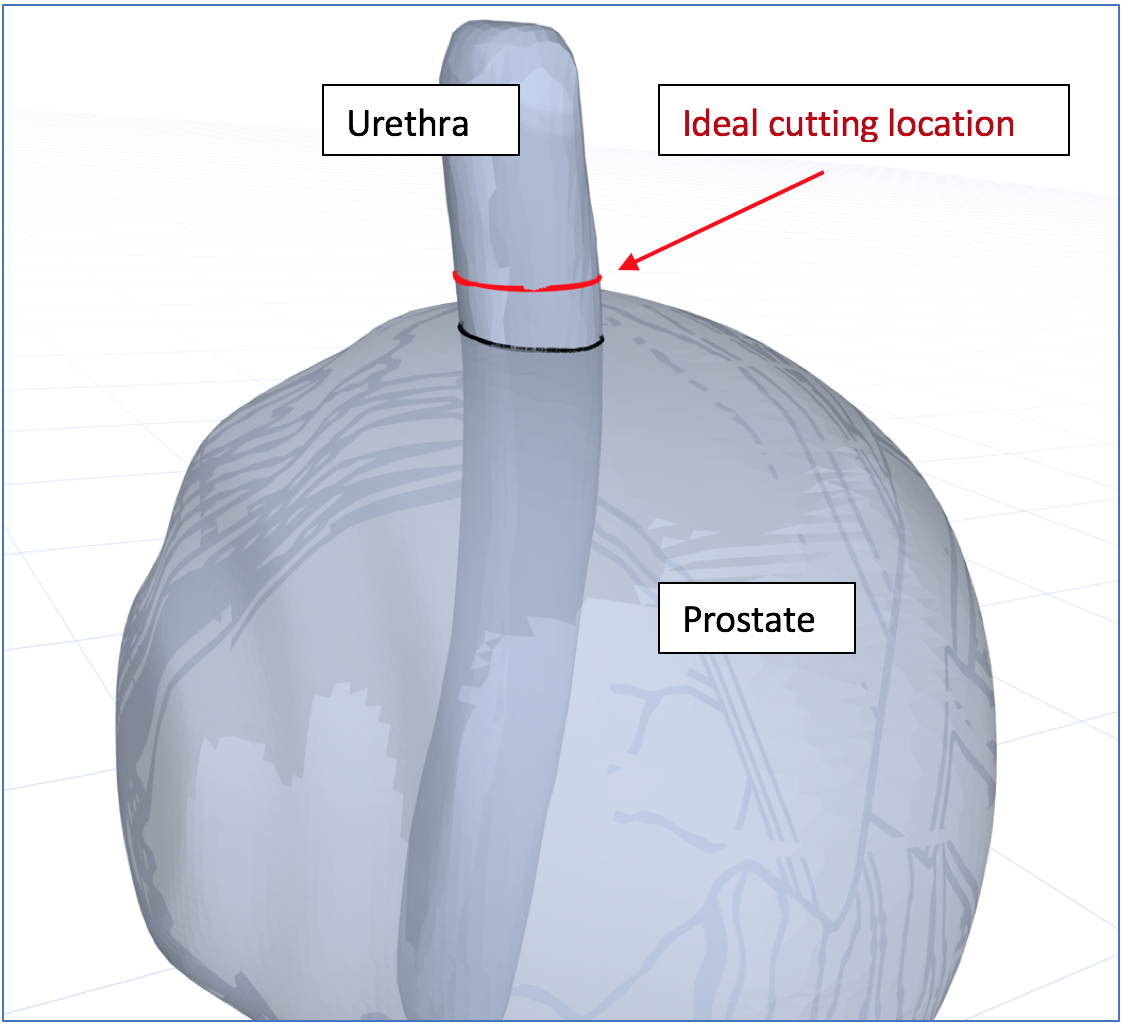
\includegraphics[width=0.5\textwidth]{validation/cut_1}
  \caption{A sketch of the interface showing the user the intended location of cutting}\label{fig:ideal_cut}
\end{figure}

\subsubsection{Shape of the Cut}
An ideal shape of the cut is evaluated by three  metrics as described in following sub-sections.

\paragraph{Cutting in One Plane}\label{par:metric_1}
This means that the cut should be symmetrical, \ie it is only performed in one plane. The plane should be parallel to the plane of the prostate surface. The simulation software should be able to calculate the cutting plane the surgeon is performing and approximate it to one flat plane parallel to the surface of the prostate for a cut to be correctly performed.
\autoref{fig:prostate_surface_plane} shows the plane of the surface of the prostate. An ideal cut should be performed in a plane parallel to this plane, as shown in \autoref{fig:cutting_location_parallel_to_prostate}. Since the training simulation will display the location of the ideal cut, as shown in \autoref{fig:ideal_cut}, a surgeon using this simulation will have a visual cue of the angle of the plane. \autoref{fig:plane_location_orientation} shows the ideal cutting plane location and orientation with respect to the plane of the prostate surface.

\autoref{fig:cutting_in_multiple_planes} show a visual representation of performing a non-uniform asymmetrical cut and how it maps to multiple planes.

\begin{figure}
  %\captionsetup[subfigure]{width=0.3\textwidth}
  \centering%
  \subbottom[The prostate's surface plane]{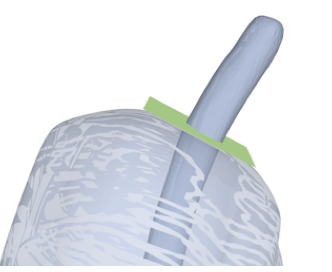
\includegraphics[width=0.3\textwidth]{validation/cut_2}\label{fig:prostate_surface_plane}}
  \hfill%
  \subbottom[The cutting location should be above the apex of the prostate and in one plane parallel to the prostate's surface plane]{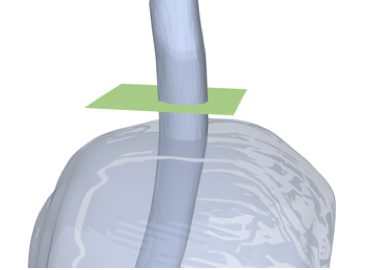
\includegraphics[width=0.3\textwidth]{validation/cut_3}\label{fig:cutting_location_parallel_to_prostate}}
  \hfill%
  \subbottom[Cutting the urethra should not be performed in a plane not in parallel to the prostate]{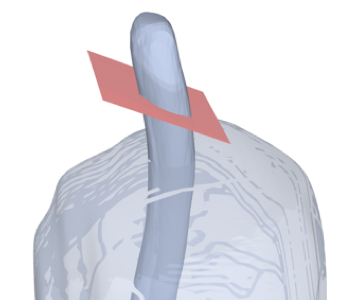
\includegraphics[width=0.3\textwidth]{validation/cut_4}\label{fig:cutting_location_not_parallel_to_prostate}}
  \caption{The ideal location and orientation of the cutting plane}\label{fig:plane_location_orientation}
\end{figure}

\begin{figure}
%\captionsetup[subfigure]{width=0.45\textwidth}
  \centering%
  \subbottom[An example of a non-uniform1 cut performed in multiple planes]{\label{fig:asymmetrical_cut}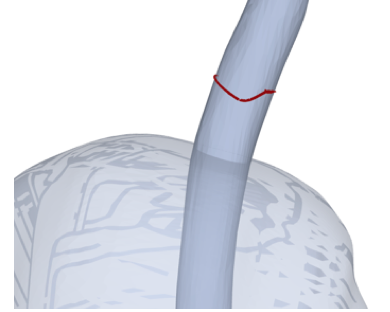
\includegraphics[width=0.45\textwidth]{validation/cut_5}}
  \hfill%
  \subbottom[Cutting the urethra should not be performed in multiple planes]{\label{fig:multiple_planes}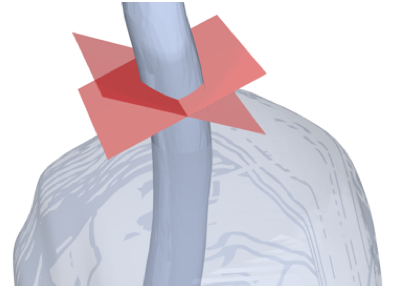
\includegraphics[width=0.45\textwidth]{validation/cut_6}}
  \caption{Cutting in multiple planes}\label{fig:cutting_in_multiple_planes}
\end{figure}

\paragraph{One Initial Opening}\label{par:metric_2}
As a good practice for a clean cut, the surgeon should should perform the task starting from only one initial cut in the urethra and should not create multiple initial cuts.

\paragraph{Cut in Small Steps}\label{par:metric_3}
Another good practice for a clean cut is cutting only a few millimeters at a time. The minimum and maximum size of a single cutting step is to be defined empirically through test runs and evaluations with surgeons during the formative validity tests.

\hrule%

\subsection{Evaluation Metrics}\label{ssec:evaluation_metrics}


% \begin{figure}
%   \centering%
% 	
\includegraphics[width=0.13\linewidth]{validation/anastomosis_blockage_1}\hspace{2ex}
% 	
\includegraphics[width=0.13\linewidth]{validation/anastomosis_blockage_2}\hspace{2ex}
% 	
\includegraphics[width=0.13\linewidth]{validation/anastomosis_blockage_3}\hspace{2ex}
% 	
\includegraphics[width=0.13\linewidth]{validation/anastomosis_blockage_4}\hspace{2ex}
% 	
\includegraphics[width=0.13\linewidth]{validation/anastomosis_blockage_5}
%   \caption{Examples of anastomosis blockage configurations.}\label{fig:anastomosis_leakage}
% \end{figure}

In order to evaluate the surgeons performance while using the simulator, several parameters need to be recorded during simulation time. These parameters are based on the aforementioned performance evaluation metrics:

\begin{enumerate}[start=1,label={Para \#\arabic*, }]
	\item \textbf{Plane of the cut:} Cutting in one symmetrical plane: The simulation software shows the user the ideal cutting plane to guide novice user. An option of hiding the ideal plane is also available for more experienced users.

	\item \textbf{Size of the cut:} small snips at a time. The size of a good cut is currently calculated by the surface area that has been separated.  If the surface area is above a certain threshold that has been empirically identified, it is considered a large cut. If it is below, it is considered a good cut. Having big snips may risk in injuring different layers that should not be cut like nerves. [] shows an illustation of big and small cuts on the simulator.

	\item \textbf{Topological cut:} The surgeon should perform the task starting from only one initial cut and continue along the same plane in the urethra and should not create multiple initial cuts. By the end of the simulation, there should exist one continuous cut around the urethra that separates it into two pieces. Whether the surgeon prefers to create one or multiple small cuts initially, they should end up as one eventually. \autoref{fig:ideal_cut} shows an illustration of initial cuts.

	\item \textbf{Rectal wall collisions:} A good practice is to avoid collisions with the surrounding tissues and rectal wall. Injuries in the rectum occur more often during the dissection of the prostatic apex (if not completely mobilized off of the posterior of the prostate). When the rectum stays adherent to the apex, it is at a risk of injury in the process of urethra transecting. \autoref{fig:recWalls} below shows the rectal wall as white-shaded areas.

\begin{figure}
  \centering%
  \subbottom[Side view of rectal wall boarders planes]{\label{fig:asymmetrical_cut}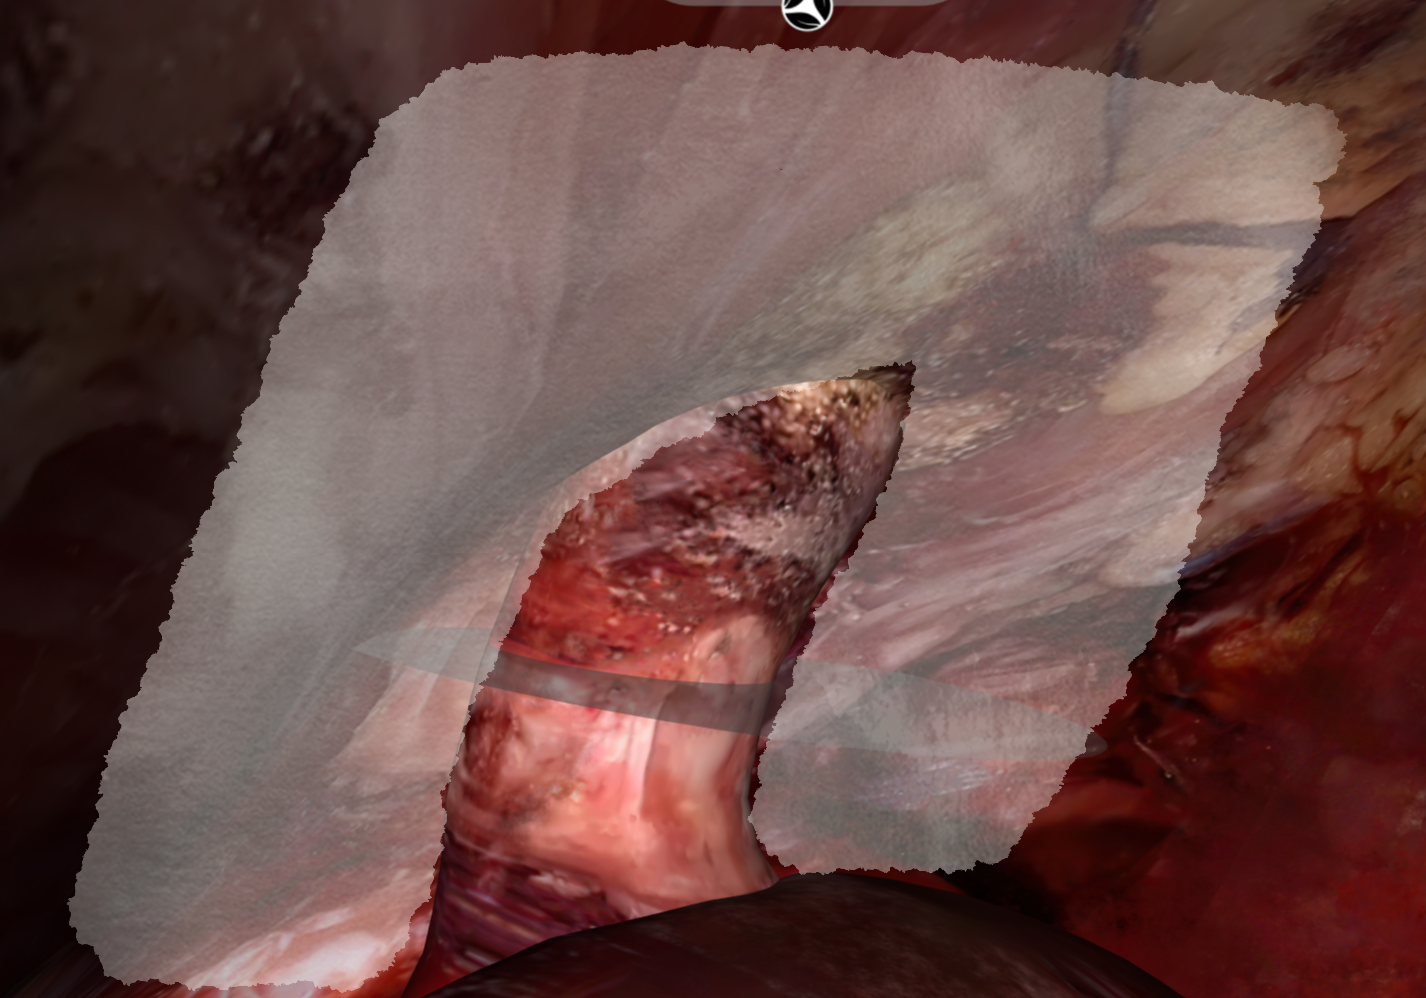
\includegraphics[width=0.45\textwidth]{figures/validation/rec1.png}}
  \hfill%
  \subbottom[Front view of rectal wall boarders planes]{\label{fig:multiple_planes}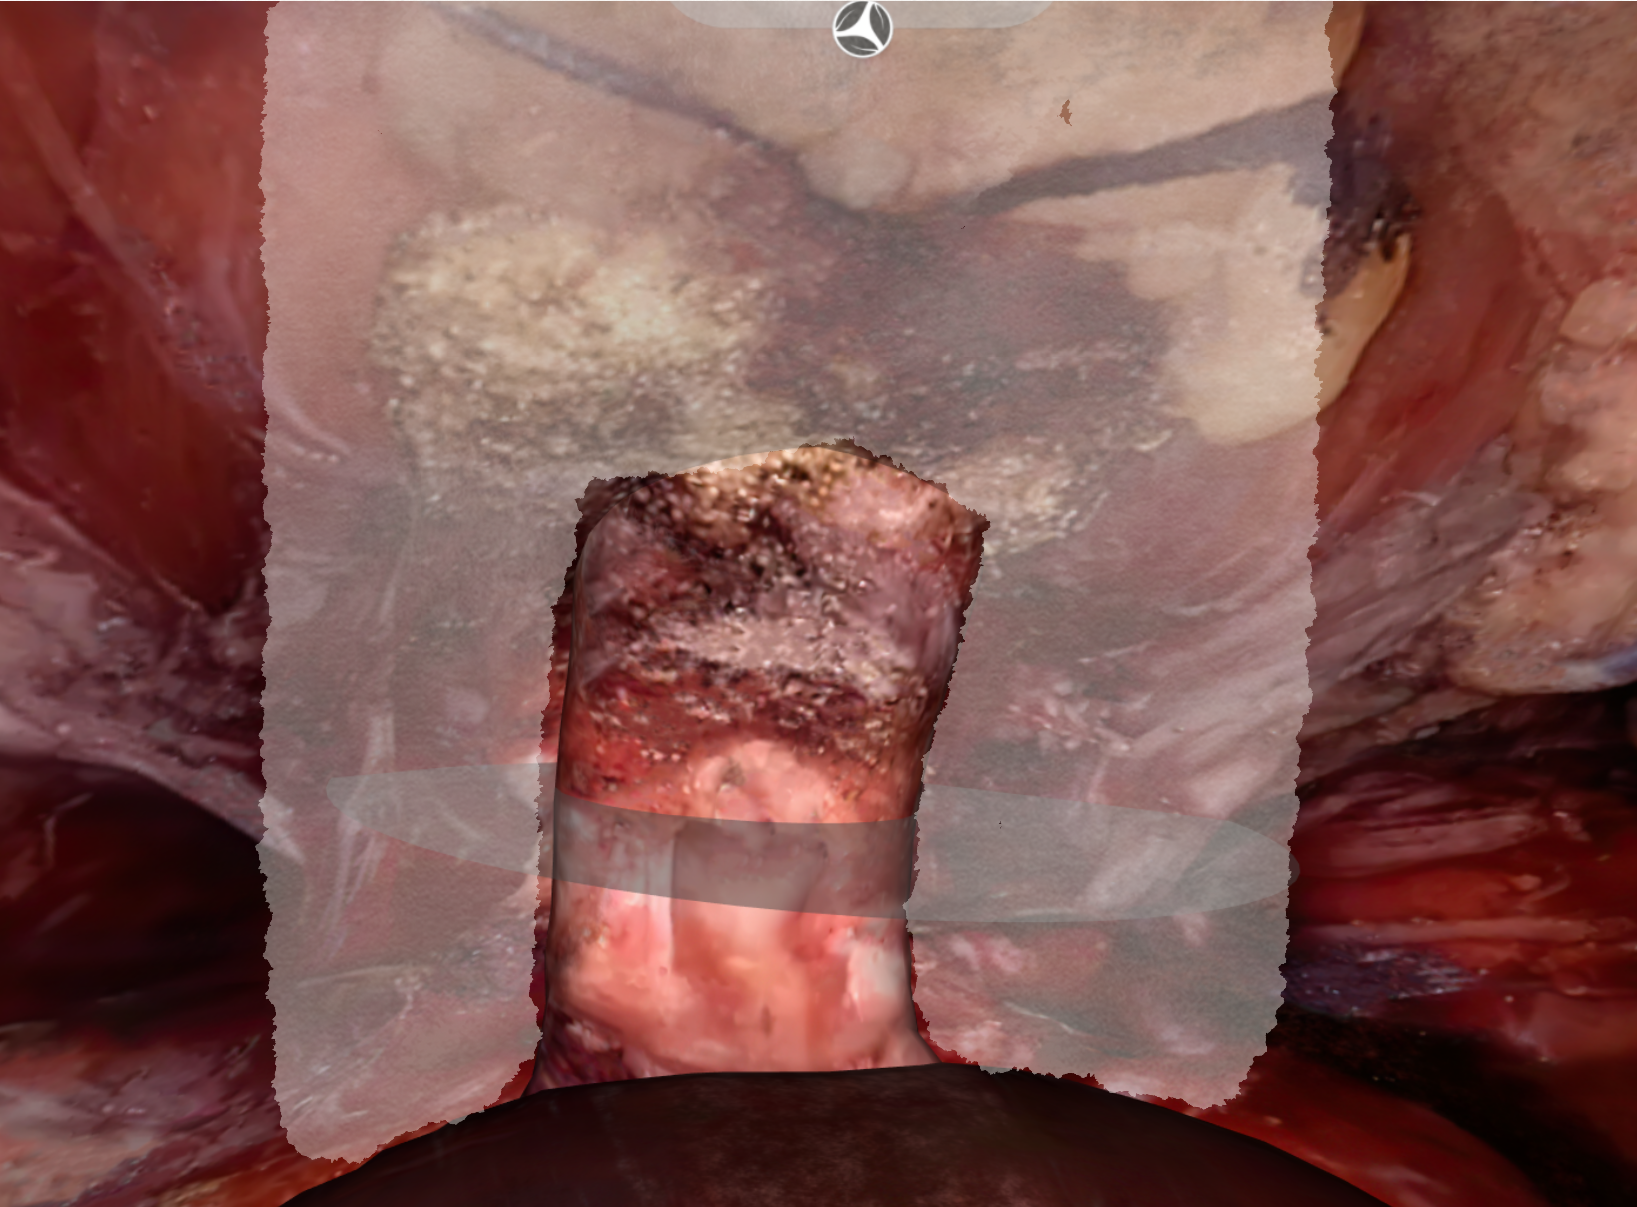
\includegraphics[width=0.45\textwidth]{figures/validation/rec2.png}}
  \caption{Rectal wall boarders}\label{fig:recWalls}
\end{figure}

	\item \textbf{Tools out-of-scene count:} A good practice is to keep surgical tools always visible within the surgical view. Moving the tools out of the scene may result in injuring the patient in a real operation setting. The surgeon shall be able to control the motion of these surgical tools and keep them within his surgical view. \autoref{fig:fov} illustrates the good and back scenarios of this parameter.

  \begin{figure}
    \centering
    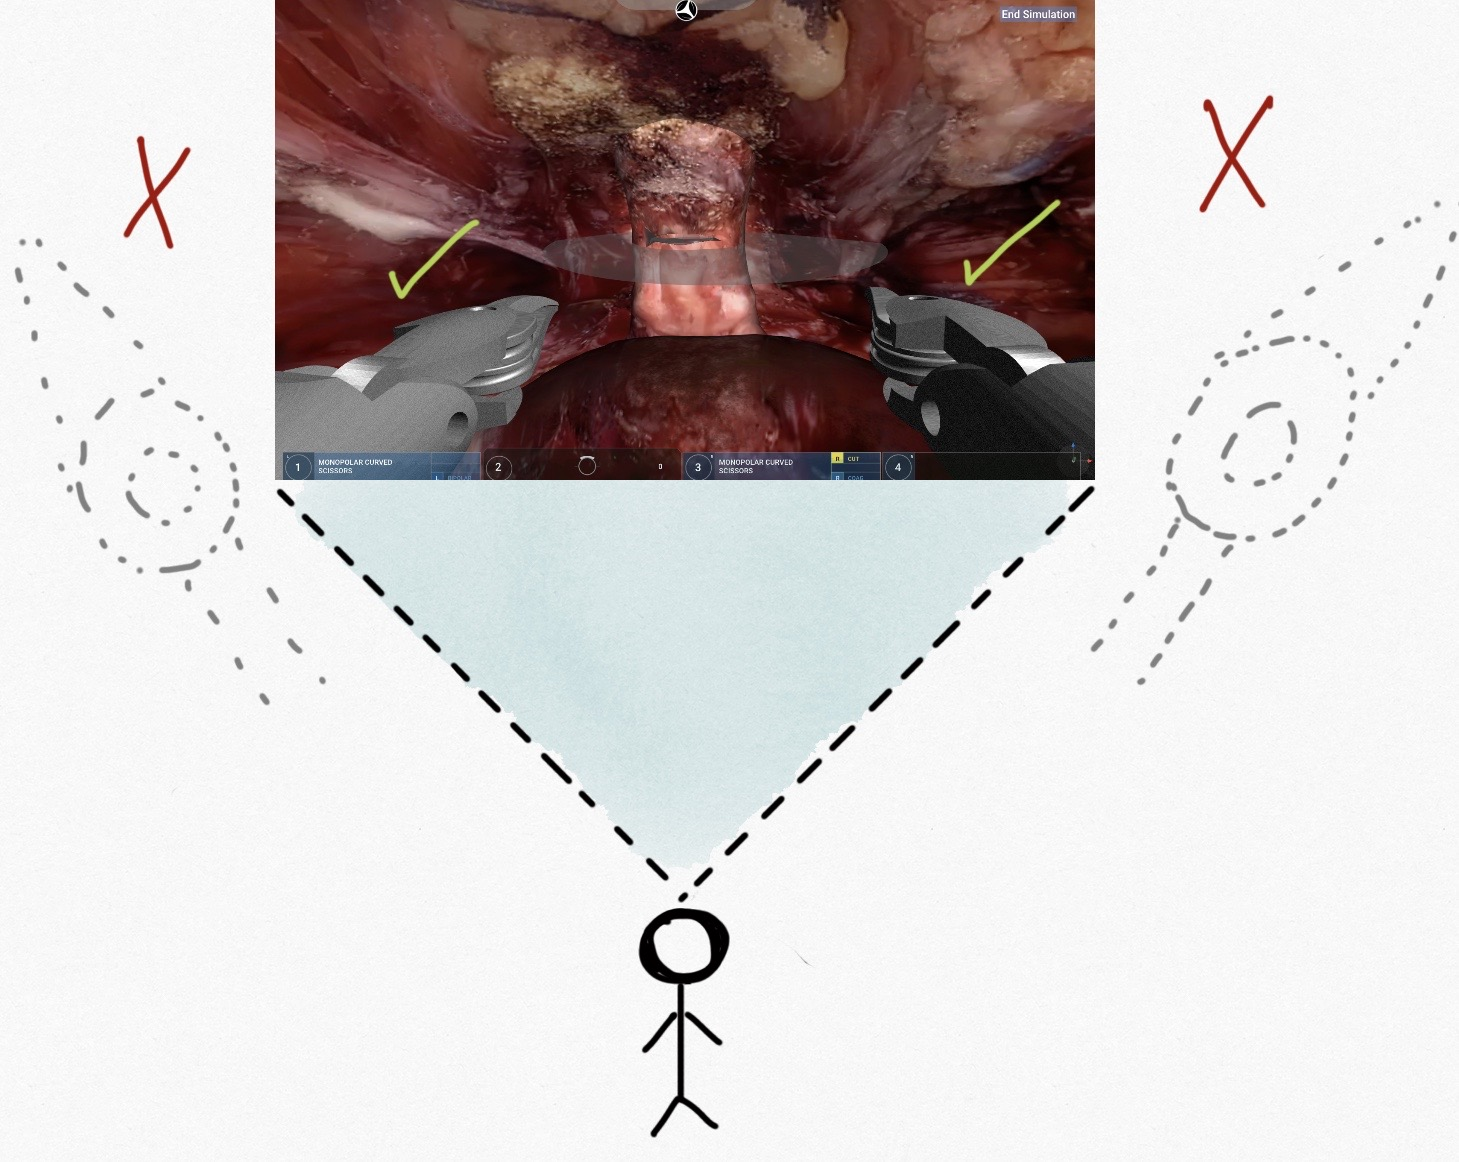
\includegraphics[width=.6\textwidth,frame]{figures/validation/fov.JPG}
    \caption{Tools should be always kept within the field of view. Tools out of the scene are dangerous in a real setting.}\label{fig:fov}
  \end{figure}

	\item \textbf{Time elapsed for task completion:} This parameter will be used to assess the skills acquired by surgeons by using this simulator through their difference in performance parameters throughout trials. This parameter will also be used as an indication to differentiate between different surgeon expertise: a senior surgeon who is used to the console set up perform the task faster than a novice surgical surgeon.
\end{enumerate}

\hrule%

\subsection{Graphical User Interface}
A graphical user interface is needed to communicate the score of the surgeon based on his or her performance in completing the cutting task and to inform the surgeon of ways to improve the performance. In this section, we present the three main screens of this simulator:
\begin{enumerate}[1.]
  \item Pre-simulation: to inform the surgeon of the scoring mechanism
  \item Simulation: to display feedback on the surgeon's performance in real-time
  \item Post-simulation: to provide an overview of the surgeon's performance and the total score
\end{enumerate}

The simulation starts with a total score of 100. The score decreases as the surgeon performs any of the following errors:
\begin{enumerate}[1.]
  \item The surgeon cuts outside the target line and ends up with an asymmetrical cut (\textbf{-10} overall)
  \item The surgeon creates more than one initial cut (\textbf{-10} per initial cut)
  \item The surgeon cuts larger than the accepted threshold per cut (\textbf{-5} per large cut)
  \item The surgeon unnecessarily collides the tool with the tissue (\textbf{-1} per collision)
  \item The surgeon's tool leaves the surgical scene (\textbf{-2} each time)
\end{enumerate}

\subsubsection{Pre-Simulation}
Before the start of the simulation, the subject is taken through a presentation about the simulator in general: the clinical problem, proposed solution, anticipated outcomes, simulator-related instructions, \etc. Then, upon the start of the simulator,a graphical user interface, presented as a mockup in \autoref{fig:pre_training_mockup}, visually presents to the surgeon instructions to correctly perform the cutting task. The first instruction (starting from the top left) is to follow the line displayed over the urethra for the ideal cutting location. The second is related to the metric presented in \autoref{par:metric_1}. The third is related to the metric presented in \autoref{par:metric_2}. The fourth is related to the metric presented in \autoref{par:metric_3}. The fifth and sixth are recommended practices in surgery to avoid collisions with tissues and to keep the tool within the field of view.
\begin{figure}
  \centering%
  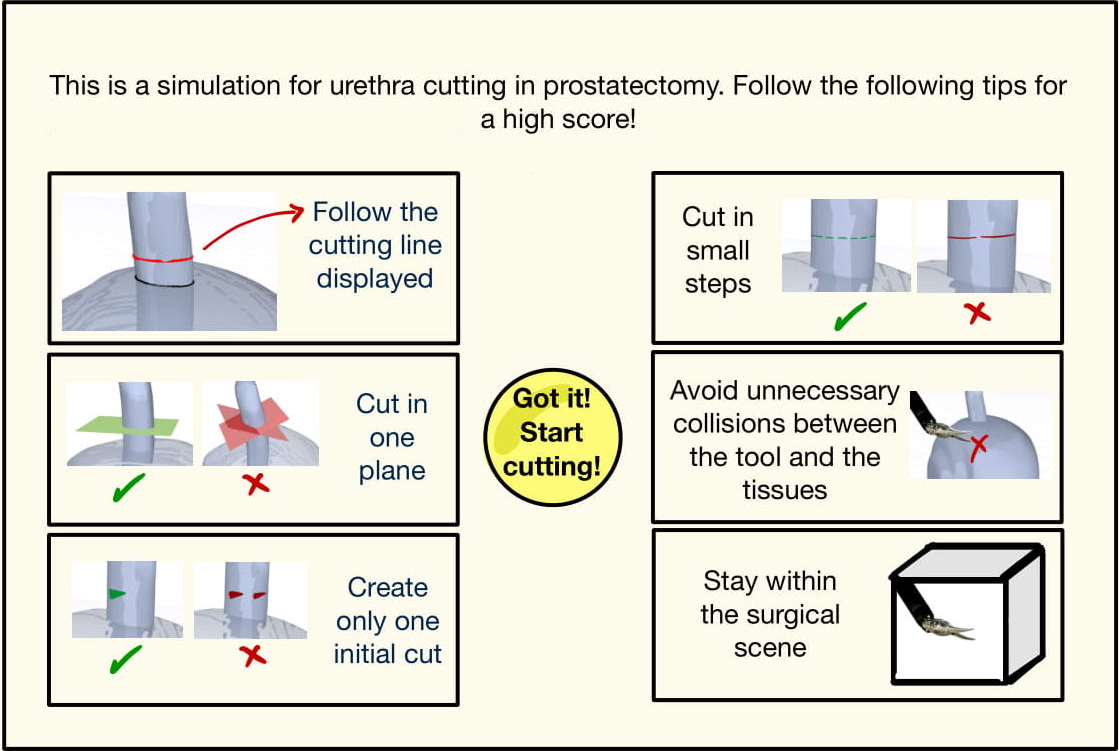
\includegraphics[width=1\textwidth]{validation/pre_training}
  \caption{A mockup of the pre-training screen}\label{fig:pre_training_mockup}
\end{figure}

\subsubsection{Per-Simulation}
This graphical user interface, presented in all its possible scenarios as multiple mockups in \autoref{fig:training_mockup}, shows the graphical representations of communicating an error to the surgeon. In the default case, the surgeon's simulator screen has little to no information displayed other than the surgical scene and the time elapsed since the start of the cutting task. In case of creating an asymmetrical cut (related to \autoref{par:metric_1}), the deviation is highlighted in red for the surgeon to visualize the cutting error and deviate back to the correct track. In case of creating multiple initial cuts (related to \autoref{par:metric_2}), the location of any other cut made other than the first one is highlighted in red. In all other error cases, a message will be displayed to the surgeon.
When the surgeon hits the rectal wall, the circumference of the simulator screen will turn red, prompting the surgeon to retract his surgical tools. In the case where the surgeon takes his tools out of the scene, a caution sign will appear indicating the exit of surgical tools and prompting the user to return them back within surgical view.
Note that all error visualizations and messages disappear within a few seconds to minimize distractions from the main task and to optimize the focus of the surgeon on cutting.
\begin{figure}
  %\captionsetup[subfigure]{width=0.45\textwidth}
  \centering%
  \subbottom[Default view]{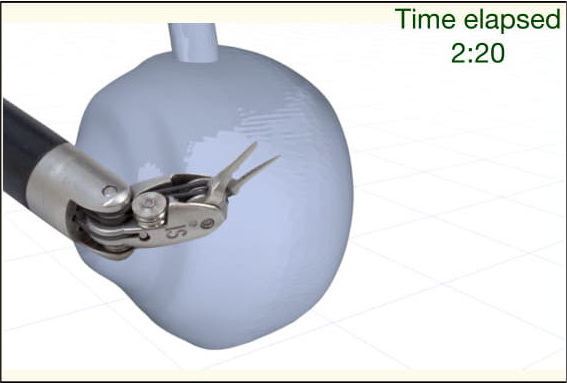
\includegraphics[width=0.45\textwidth]{validation/training_1}}
  \hfill%
  \subbottom[Error: asymmetrical cut]{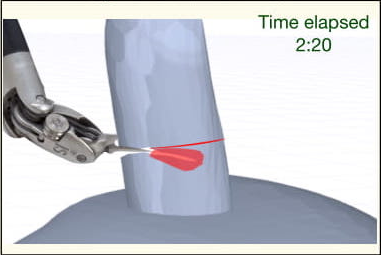
\includegraphics[width=0.45\textwidth]{validation/training_2}}
  \\
  \subbottom[Error: multiple initial cuts]{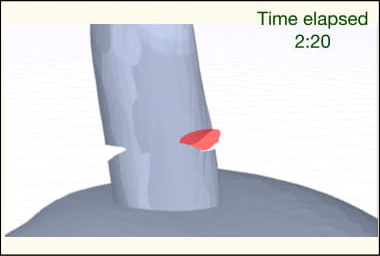
\includegraphics[width=0.45\textwidth]{validation/training_3}}
  \hfill%
  \subbottom[Unnecessary collusion with surrounding organs]{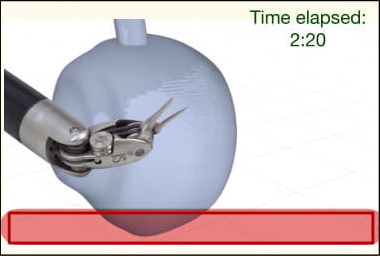
\includegraphics[width=0.45\textwidth]{validation/training_4}}
  \caption{A mockup of the training screen and the different possible scenarios}\label{fig:training_mockup}
\end{figure}

\subsubsection{Post-Simulation}
This graphical user interface, displayed upon the completion of the cutting task, displays to the surgeon the total score as well as a breakdown of the errors performed during the task. An example is presented in the mockup in \autoref{fig:post_training_mockup}. In this example, the surgeon has scored a total of 76\%, with an asymmetrical cut, two instances of large cuts, and four unnecessary collisions between the tool and the tissue. The interface also displays to the user options to repeat the task or exit the simulation.
\begin{figure}
  \centering%
  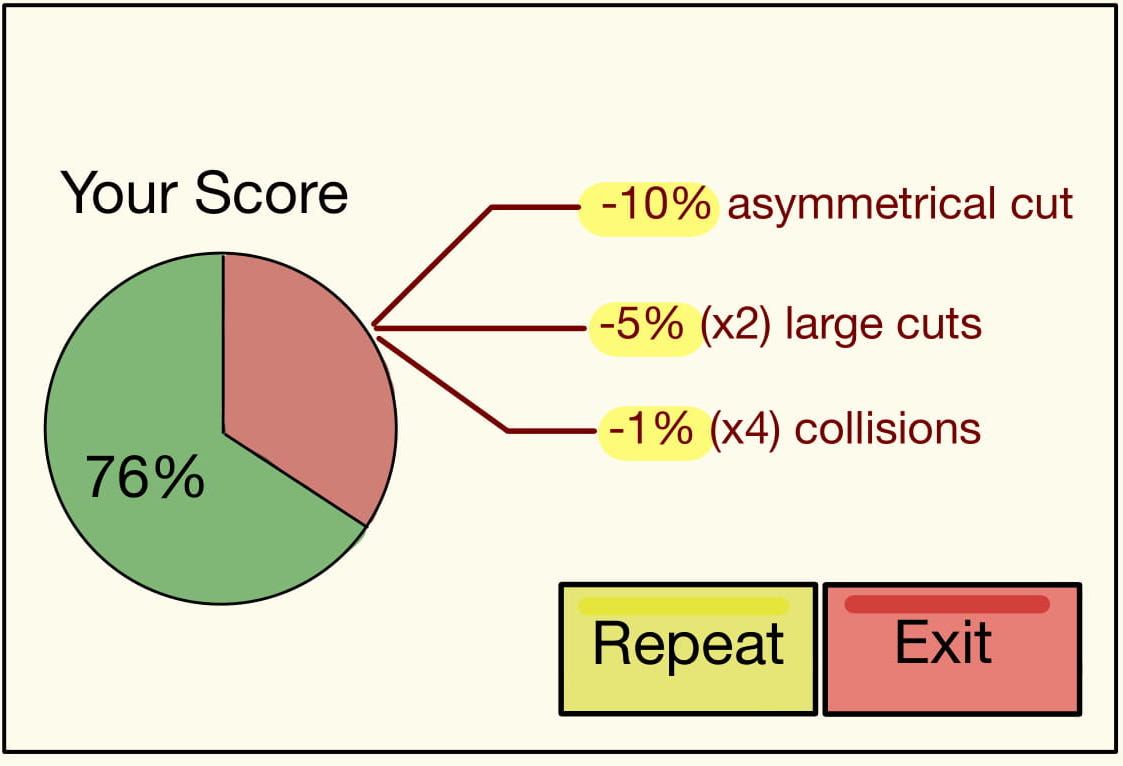
\includegraphics[width=.7\textwidth]{validation/post_training}
  \caption{A mockup of an example of results screen}\label{fig:post_training_mockup}
\end{figure}

\subsection{Evaluation Protocol}

The validity tests we performed during the development stage of the project are carried in a form of a formative usability study. A formative usability study is an iterative process of multiple usability testing approaches to evaluate the system being developed and assess the integration of features to ensure detecting and eliminating usability issues early before the final design is produced.

Formative evaluation focuses on qualitative results collected from a variety of evaluators, including the design and development team, experts in the field, and target users. In the case of our simulation interface, participants in formative evaluations include the research team, expert surgeons, surgery training professionals, medical doctors with a background in prostatectomy, and surgeons-in-training. These methods are tailored to focus on the face, content and construct parameters of the simulator.

The data collected from the described formative usability testing methods is primarily qualitative.  This data can be later categorized into areas of improvement and used to enhance the simulator for running the next iterations of formative evaluation tests. This qualitative data describes the state of each of the heuristics for face, content and construct validity and list usability issues to be resolved and areas of improvement.

We conducted two formative evaluation tests: heuristics evaluation and think-aloud evaluation.

Once a significant set of features are added to the prototype, a proper usability evaluation with both qualitative and quantitative data is performed. Qualitative data becomes crucial to objectively quantify the surgeon performance rather than getting subjective qualitative feedback.


Towards the end of the project, summative usability study is performed. Summative study is quantitative evaluation with representative users where they are required to perform usability studies, collect their performance measures and perform statistical analysis. This test is mainly done before the end of the project to compare it with initial requirements and test its overall usability.

\subsubsection{Heuristics Evaluation}
Heuristics evaluation is a formative evaluation method for finding the highest number of usability issues before the final design is produced. A list of heuristics is generated and tested through using the system of interest by a group of evaluators.

\paragraph{Study Participants}
For formative study, the participants (or evaluators) are not the target users, but usability experts and domain experts. A diverse group of evaluators ensures finding different types of and more usability issues. In the case of this project, this includes expert surgeons (whom this project is not targeted for, but can provide insights on the usability of the interface), the research team, and medical doctors with a background in prostatectomy.

In summative study, targeted users (end users) are asked to perform these evaluations, while focusing on quantitative analysis. Targeted users for this project are medical doctors who are training on how to use the DaVinci console.

\paragraph{Study Structure}
In heuristics evaluation, evaluators participate in two sessions: individual and group. In the individual session, the evaluator performs the cutting task and discusses a number of heuristics with the test moderator or the main usability researcher. In the group session, evaluators discuss their individual findings and propose solutions to these problems. The following is the detailed structure of each session.

\subparagraph{Individual Evaluation Session} A session for where the evaluator individually completes and discusses the cutting task with the test moderator.
\begin{enumerate}[1.]
  \item Introduction (standardized with all evaluators):
  \begin{enumerate}[\em a\em)]
  \item Provide an overview of the project and the heuristics evaluation method,
  \item Describe the current state and capabilities of the system,
  \item Describe (and demo, if necessary) the cutting task.
  \end{enumerate}
  \item Allow the evaluator to freely use and explore the interface,
  \item Guide the evaluator through the task, while discussing the heuristics,
  \item Record the usability problems encountered or reported by the evaluator.
\end{enumerate}

\subparagraph{Group Debriefing Session}
After individually testing with all the evaluators, organize a group meeting, list all the problems encountered with all evaluators, and discuss possible solutions.

\paragraph{Cutting Task Heuristics}
\begin{enumerate}[1.]
  \item Face Validity:
	\begin{enumerate}[\em a\em)]
	  \item The cutting mechanism represents a real world cutting task in a prostatectomy surgery
	  \item The device is a sufficiently accurate representation of a real robotic system
	  \item The hand controllers are effective for working in the simulated environment
	  \item The user interface is efficient and minimalistic
	\end{enumerate}

  \item Content Validity:
	\begin{enumerate}[\em a\em)]
	  \item The cutting task is effective for teaching the cutting skill for our target users
	  \item The scoring system effectively communicates the user's performance on the cutting exercise
	  \item The scoring system effectively guides the user to improve the performance on the simulator
	  \item The scoring system is effectively communicated to the user and messages are presented in plain language
	  \item Learning the system is feasible by first-time users with minimal supervision/training
	\end{enumerate}

  \item Construct Validity:
	\begin{enumerate}[\em a\em)]
	  \item The system is able to distinguish between an experienced and a novice user based on errors
	  \begin{enumerate}[\em i\em)]
	    \item Number of times the cutting tool damages the tissue with unnecessary touches/cuts
	    \item Number of times the cutting tool goes outside the defined boundary
	  \end{enumerate}
	  \item The system is able to distinguish between an experienced and a novice user based on shape of cut
	  \begin{enumerate}[\em i\em)]
		  \item An interpolated plane of the overall cut (with a threshold for error tolerance)
		  \item The number of centimeters per small cut
		  \item The number of initial cuts
	  \end{enumerate}
	  \item The system is able to distinguish between an experienced and a novice user based on general statistics
	  \begin{enumerate}[\em i\em)]
		  \item Time taken to complete the test
	  \end{enumerate}
  \end{enumerate}
\end{enumerate}

\subsubsection{Think-aloud Evaluation}
Contrary to heuristics, the think-aloud method is performed with target users. In this method, the only data collected from the user is their thinking process throughout using the simulation and while completing the cutting task. Also, contrary to heuristics, the test moderator does not interfere or discuss the interface with the participant. Similar to heuristics, task completion is performed individually. This method is performed in three simple steps:

\begin{enumerate}[1.]
  \item Recruit representative subjects (target users)
  \item Ask the subjects to complete the cutting task and describe their mental process as they complete the task
  \item Meanwhile, the test moderator records the session and takes note of the interaction
\end{enumerate}

Following the session, the subjects filled a qualitative evaluation form including Likert-scale questions relating to face and content validity and discussed the interface informally with the team.

\hrule%

Based on the heuristic evaluation protocol, we prepared a questionnaire on a Likert Scale of 1 to 5, with 1 being \enquote{Strongly Disagree} to 5 being \enquote{Strongly Agree,} to validate and assess the simulator for face and content validity. The questions on Likert Scale will assist in assessing:
\begin{enumerate}[\em i\em)]
  \item The subjective realism of the simulator, \ie the face validity, and
  \item Its appropriateness as a teaching modality, \ie the content validity.
\end{enumerate}

The questionnaire was provided to the evaluators after allowing them to freely use and interact with the cutting simulator. While using the cutting simulator, they were engaged in a discussion with the validity test moderator to assess the usability. Information about the participants (\emph{evaluators}) was collected. This enable classification of the feedback based on the experience level and specialization of the evaluator.

Secondly, we have started implementation of the clinical metric for logging user interactions to assess construct validity. We have identified the information, described in Aim 5: Training and Test Scenarios, to be logged during the interaction of the evaluator with simulator. The information will be displayed after the completion of the task, as displayed in the graphical user interface described in Aim 5: Training and Test Scenarios.

We have attached the following:
\begin{enumerate}[1.]
  \item A document used to collect information related to validation studies focusing on face and content validity (\autoref{apn:questionnaire}),
  \item A summary of the scoring based on aforementioned questionnaire and feedback collected during the study (\autoref{apn:responses}), and
  \item A report describing implementation of logging mechanism for construct validity (\autoref{apn:logging}).
\end{enumerate}

\hrule
Estimated time: 10 minutes\\[-2ex]
\hrule%
The session moderator starts by taking permission for voice or video recording for future research use exclusively and letting them know that this session would take approximately one hour.  explaining the background of the surgical simulation with respect to urethral dissection and the technology under development. Moderator would use appropriate tools like a presentation and a RARP video. Using the Think-aloud protocol, the surgeon is then asked to loudly express all their thoughts about the simulator, whether they are positive or negative. The surgeon is later asked to fill in a form with information such as name, speciality, number of experience years, \etc.

\subsection{Evaluation session}
Estimated time: 30 minutes\\[-2ex]
\hrule%
During this session, the subject will manipulate simulated model using the provided interface to get familiar with the setup at first, Then, the subject will start the snipping the tubular structure (representing urethra) and the user-interactions will be logged.
While performing the snipping, the subject is expected to speak out their thoughts, while the moderator is asking them questions to get further feedback. The moderator shall remain unbiased while asking questions.
A subject is expected to perform the same action (small snips on the urethra until it is completely detached in two pieces) five times.
A unique identifier (ID) is assigned to each subject to preserve their anonymity. Since the procedure is repeated five times, the ID is assigned as follows, for instance: \texttt{50\_1}, \texttt{50\_2}, \texttt{50\_3}, \texttt{50\_4}, \texttt{50\_5}. \autoref{fig:subject} below shows the experimental setup during one of the evaluation studies:

\begin{figure}
  \centering
  \includegraphics[width=.7\textwidth,frame]{figures/validation/subject.jpeg}
  \caption{A urologist while performing the cutting task}
  \label{fig:subject}
\end{figure}

\subsection{Post evaluation session}
Estimated time: 20 minutes\\[-2ex]
\hrule%
Once the subject finishes all five trials, the moderator asks him to fill in some questions related to face and content validity. They are also free to express any further feedback that was not addressed through the questionnaire.

\hrule%

\subsection{Validation and Assessment}

Based on the evaluation protocol, a questionnaire was prepared using Likert Scale of 1 to 5, with 1 being \enquote{Strongly Disagree} to 5 being \enquote{Strongly Agree} to assess the simulator. Before the start of the simulation, information about subjects are collected to enable the classification of feedback based on the experience level and the specialization of the subject. Another questionnaire will be provided to the evaluators after allowing them to freely use and interact with the cutting simulator. While using the cutting simulator, they will be engaging in a discussion with the validity test moderator to assess the usability of the interface. Attached is a document (\autoref{apn:evaluation_questionnaire}) with questions that were used to collect information related to validation studies of face and content.



\hrule%

% TO BE DELETED: \section{Metrics for Performance Evaluation}\label{part:}

% This document includes the technical details for collecting metrics to evaluate the user's performance in the surgical simulator built for the project.

\subsection{List of Variables and Log Files}

The types of variables logged are classified into three categories, resulting in  total of three log files to be generated for a cutting task:

\begin{enumerate}[1.]
  \item \textbf{Per Cut}: Data recorded after a single cut is completed. In the case of scissors, a single cut is defined from when the scissors open ($t_1$) near a mesh to when the scissors close ($t_2$), resulting in mesh deformation. In the case of a single blade, a single cut is defined from when a blade collides with a mesh ($t_1$), to when it is moved away from the mesh ($t_2$), resulting in mesh deformation. %\footnote{NOTE: The ‘mesh deformation’ for current implementation only includes cutting and no FEM, \ie data is logged before ($t1$) and after ($t2$) cut is made. If FEM is implemented, then the data will be logged before cutting ($t1$), after cutting ($t2$), and after FEM computations are done($t3$). }
  \item \textbf{Per Collision}: Data recorded at each collision between the tool and the mesh of interest.
  \item \textbf{Per Time Frame}: Data recorded at all times.
\end{enumerate}

Here is a list of all the values to be collected from a running program. Later sections include detailed descriptions of each.

\subsubsection{Variables Recorded Per Cut}

\begin{itemize}[\tiny$\blacksquare$]
  \item $A^t_{predef}$: Cut Area Pre Deformation (Top)
  \item $A^b_{predef}$: Cut Area Pre Deformation (Bottom)
  \item $A^t_{postdef}$: Cut Area Post Deformation (Top)
  \item $A^b_{postdef}$: Cut Area Post Deformation (Bottom)
  \item Plane Inclination and Distance Statistics
	  \begin{enumerate}[1.]
	    \item $dMin_{predef}^t$
	    \item $dMax_{predef}^t$
	    \item $dMed_{predef}^t$
	    \item $dMin_{predef}^b$
	    \item $dMax_{predef}^b$
	    \item $dMed_{predef}^b$
	    \item $dMin_{postdef}^t$
	    \item $dMax_{postdef}^t$
	    \item $dMed_{postdef}^t$
	    \item $dMin_{postdef}^b$
	    \item $dMax_{postdef}^b$
	    \item $dMed_{postdef}^b$
	  \end{enumerate}
  \item Initial Cut Counter
  \item Swipe Area of Blades
  \begin{enumerate}[1.]
	  \item Case I: Single Blade
	  \item Case II: Scissors
  \end{enumerate}
\end{itemize}

\subsubsection{Variables Recorded Per Collision}
\begin{itemize}[\tiny$\blacksquare$]
  \item Unnecessary Collisions Counter
\end{itemize}

\subsubsection{Variables Recorded Per Time Frame}
\begin{itemize}[\tiny$\blacksquare$]
  \item Coordinates and Angles of Blades
  \item Surgical Scene Exit Counter
\end{itemize}

\subsection{Variables for Scoring}

\subsubsection{Cut Area: $A^t_{predef}$, $A^t_{postdef}$, $A^b_{predef}$, $A^b_{postdef}$}
\label{para:data_cut_area}

This variable describes the area of the surfaces formed at the site of the cut. As shown in Figure \ref{fig:cut_area}, when a tetrahedral $x$ is cut, a new small surface is formed at the top ($a^t_x$) and at the bottom ($a^b_x$). A surface formed with an entire cut ($A$) is a summation of a total of $N$ small surfaces created at that site. This applies to the top ($A^t$) and bottom ($A^b$) areas of a cut, where:

\[ A^t = \sum_{i=1}^{N}a^t_i \]
\[ A^b = \sum_{i=1}^{N}a^b_i \]

\begin{figure}
  \centering%
  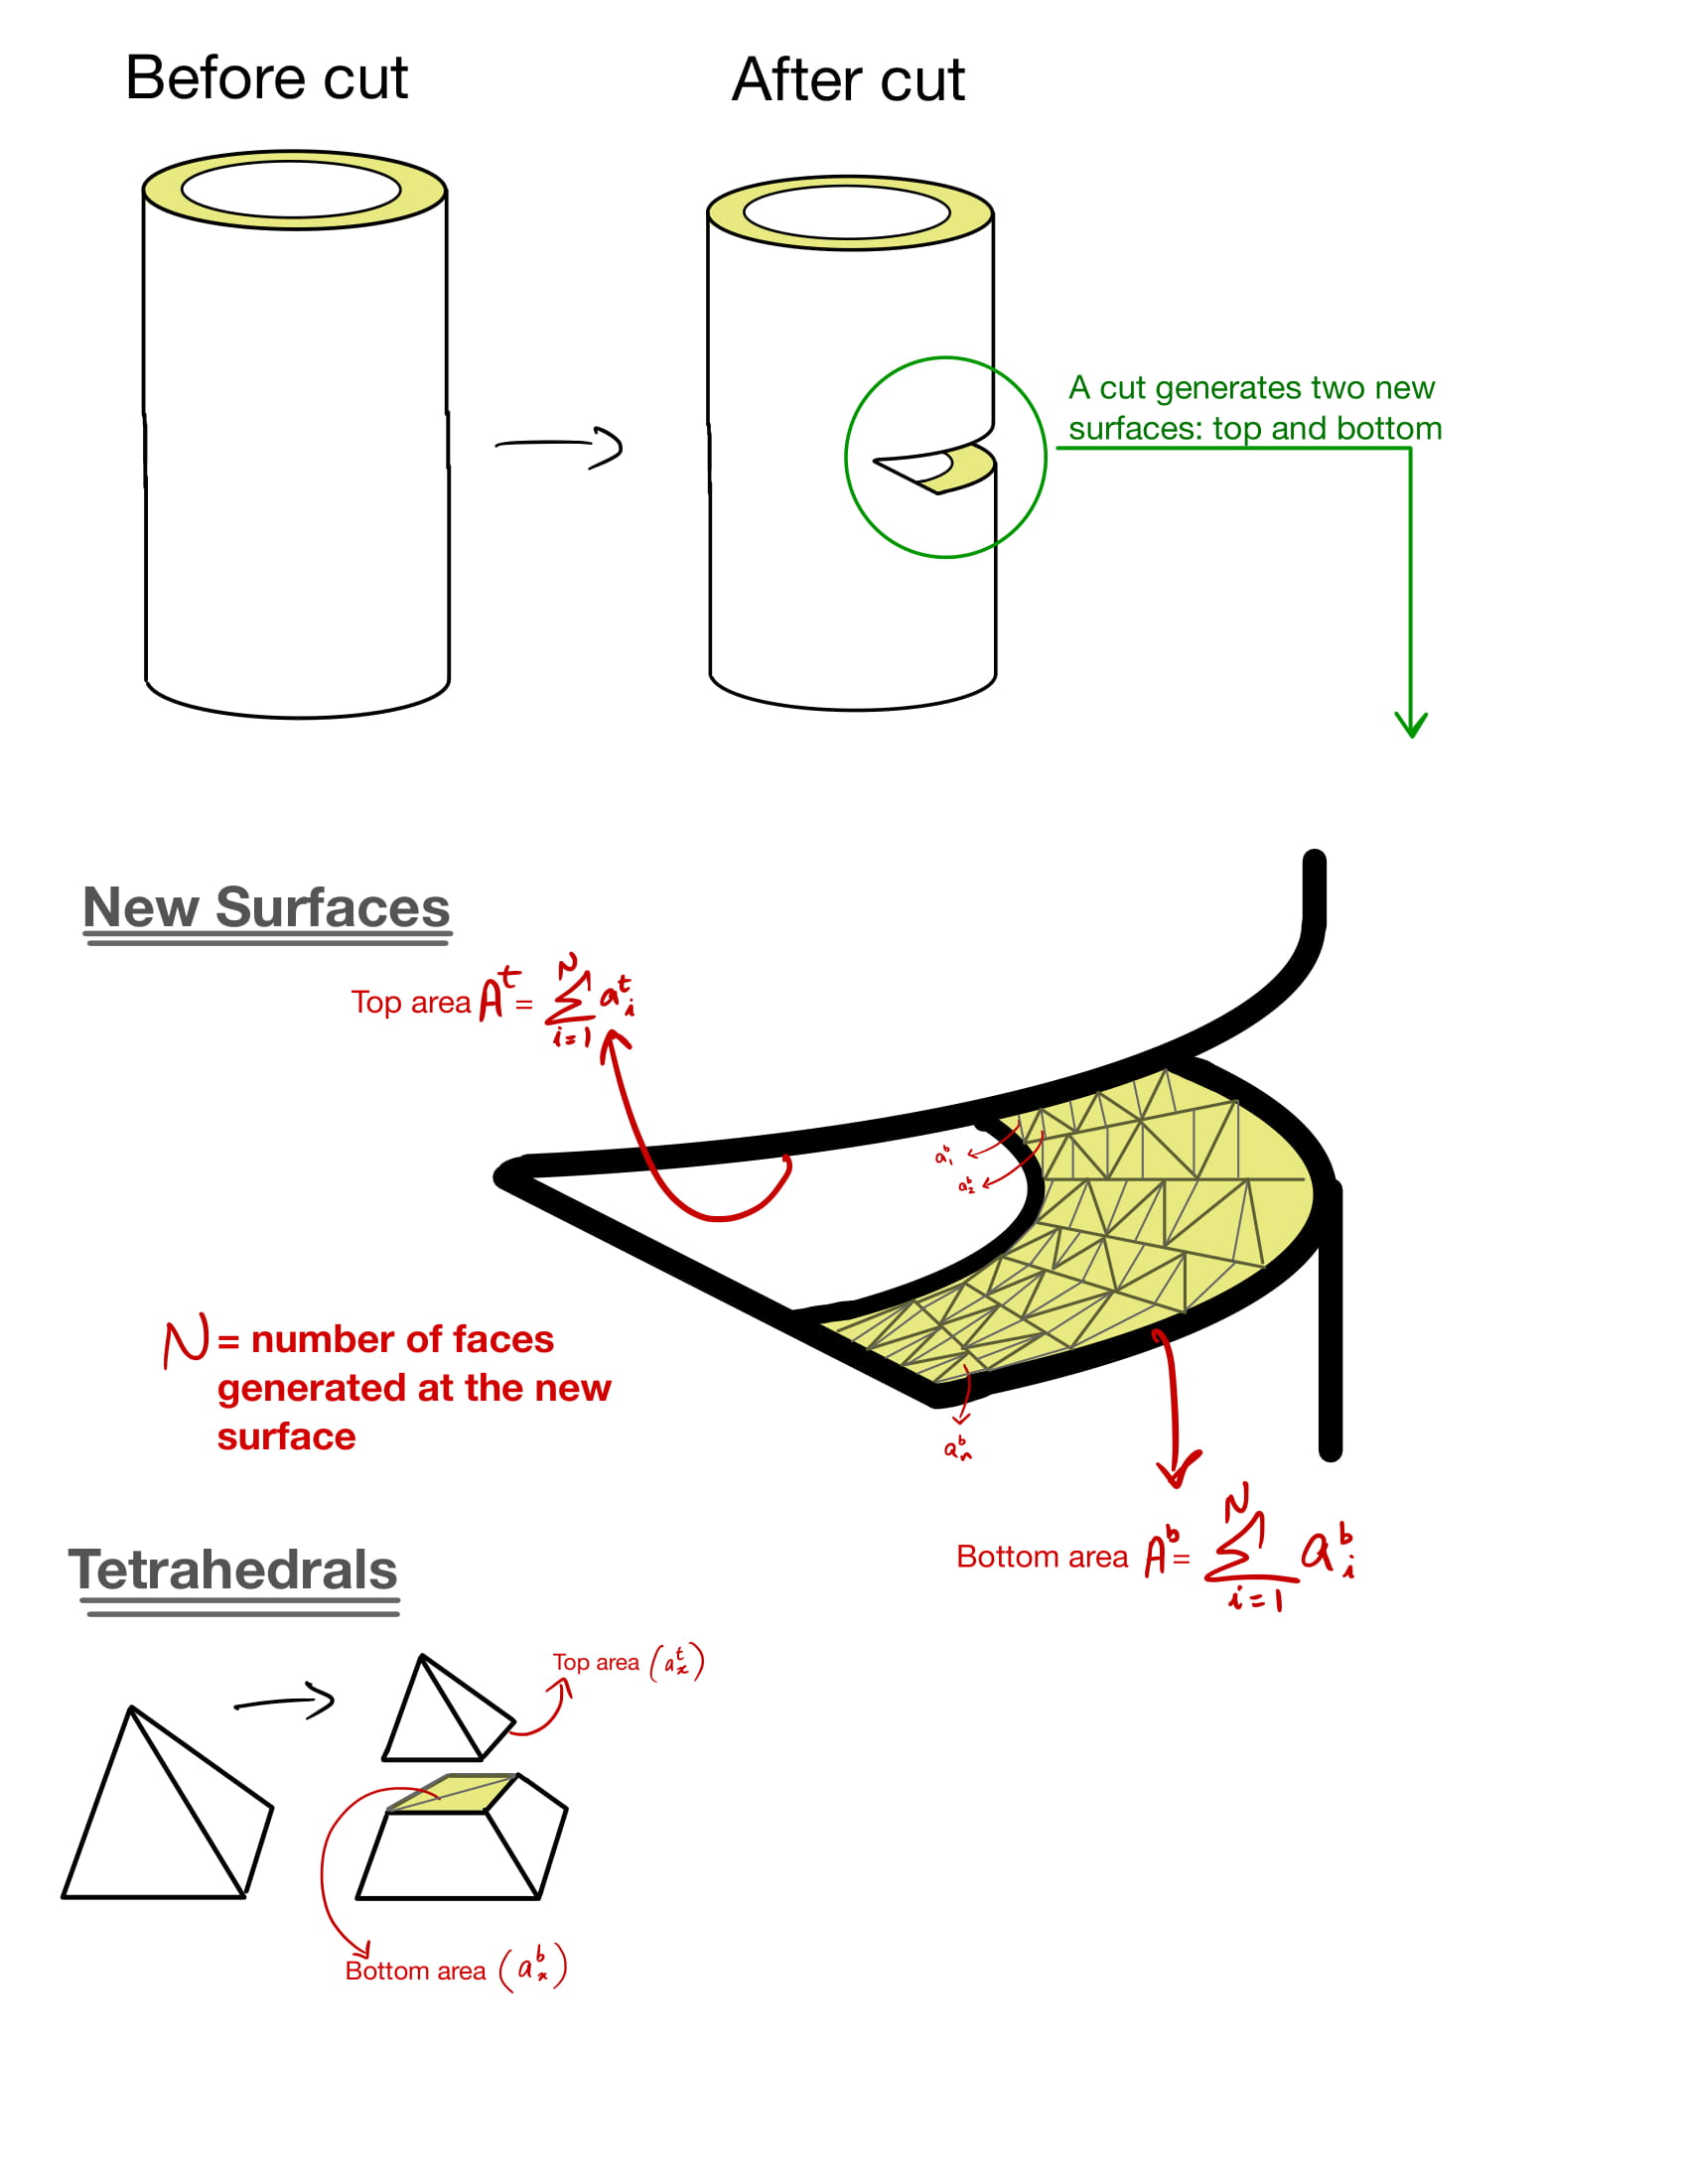
\includegraphics[width=0.6\textwidth]{validation/cut_area.jpg}
  \caption{Cut Area Variable Description}\label{fig:cut_area}
\end{figure}

These variables are recorded before deformation ($predef$) and after deformation ($postdef$).

\subsubsection{Plane Inclination And Distance Statistics}\label{para:data_plane_inclination_and_distance}

To assess the shape of the cut, it is compared in real time to an ideal (invisible) cutting plane. As shown in \autoref{fig:surface_to_plane_distance}, the distance between each vertex and the plane is calculated as $d_1$, $d_2$ and $d_3$ per triangle. The data logged per cut is the minimum ($dMin$), maximum ($dMax$), and median ($dMed$) of all the generated distances for all the vertices of the new surface. Given that each cut results in two surfaces (top $t$ and bottom $b$), the distances are calculated separately per surface, resulting in the following variables for logging after each cut. Similarly, these values are logged before and after deformation.

\hfill

$dMin_{predef}^t$, $dMax_{predef}^t$, $dMed_{predef}^t$, $dMin_{predef}^b$, $dMax_{predef}^b$, $dMed_{predef}^b$

\hfill

$dMin_{postdef}^t$, $dMax_{postdef}^t$, $dMed_{postdef}^t$, $dMin_{postdef}^b$, $dMax_{postdef}^b$, $dMed_{postdef}^b$

\begin{figure}
  \centering%
  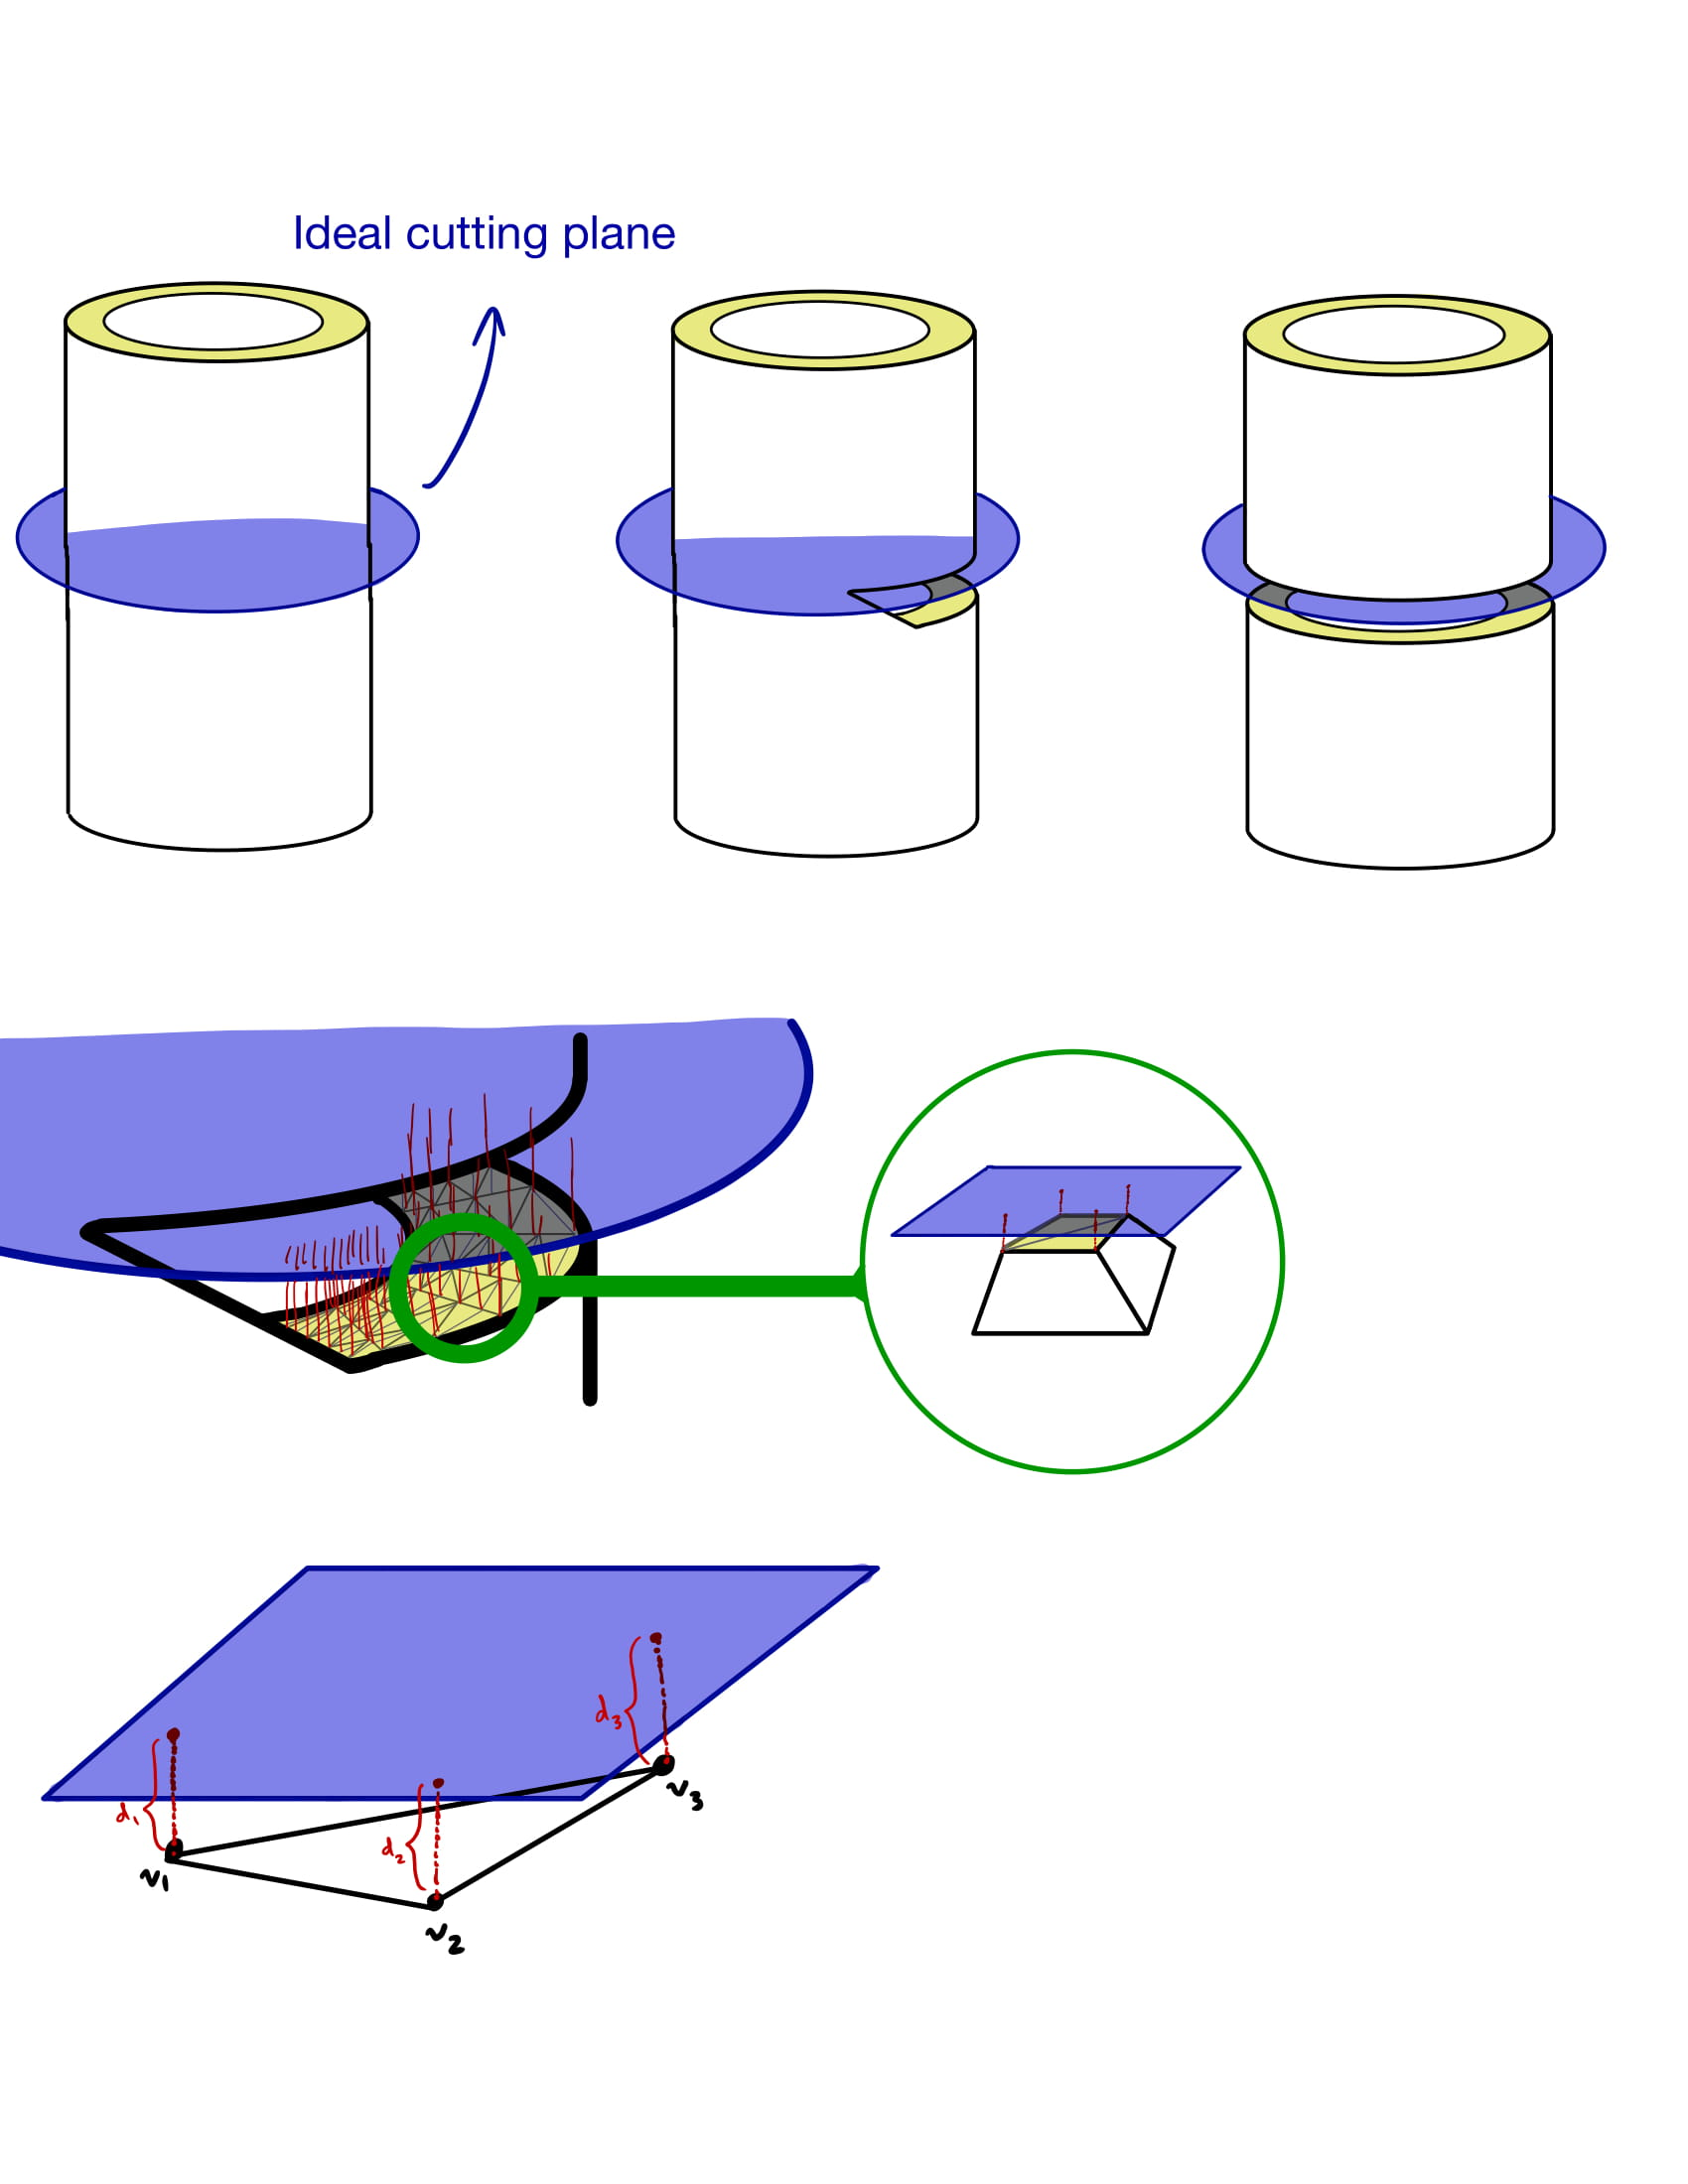
\includegraphics[width=0.7\textwidth]{validation/plane_distance.jpg}
  \caption{Surface to Plane Distance}\label{fig:surface_to_plane_distance}
\end{figure}

\subsubsection{Counters}\label{para:data_counters}

\paragraph{Initial Cut}\label{para:data_counters_initial_cut}

For a cut to be correct, the total number of initial cuts should not exceed 1. A way to determine the number of cuts is by flagging all the tetrahedra nearby a newly-generated surface with a boolean variable. After each cut:

\begin{itemize}
\item If the tool had an initial collision with a non-flagged tetrahedral, increase the counter $InitialCutCounter$ by one.
\item If the tool had an initial collision with a flagged tetrahedral, keep the counter value $InitialCutCounter$ the same.
\end{itemize}

\begin{figure}
  \centering%
  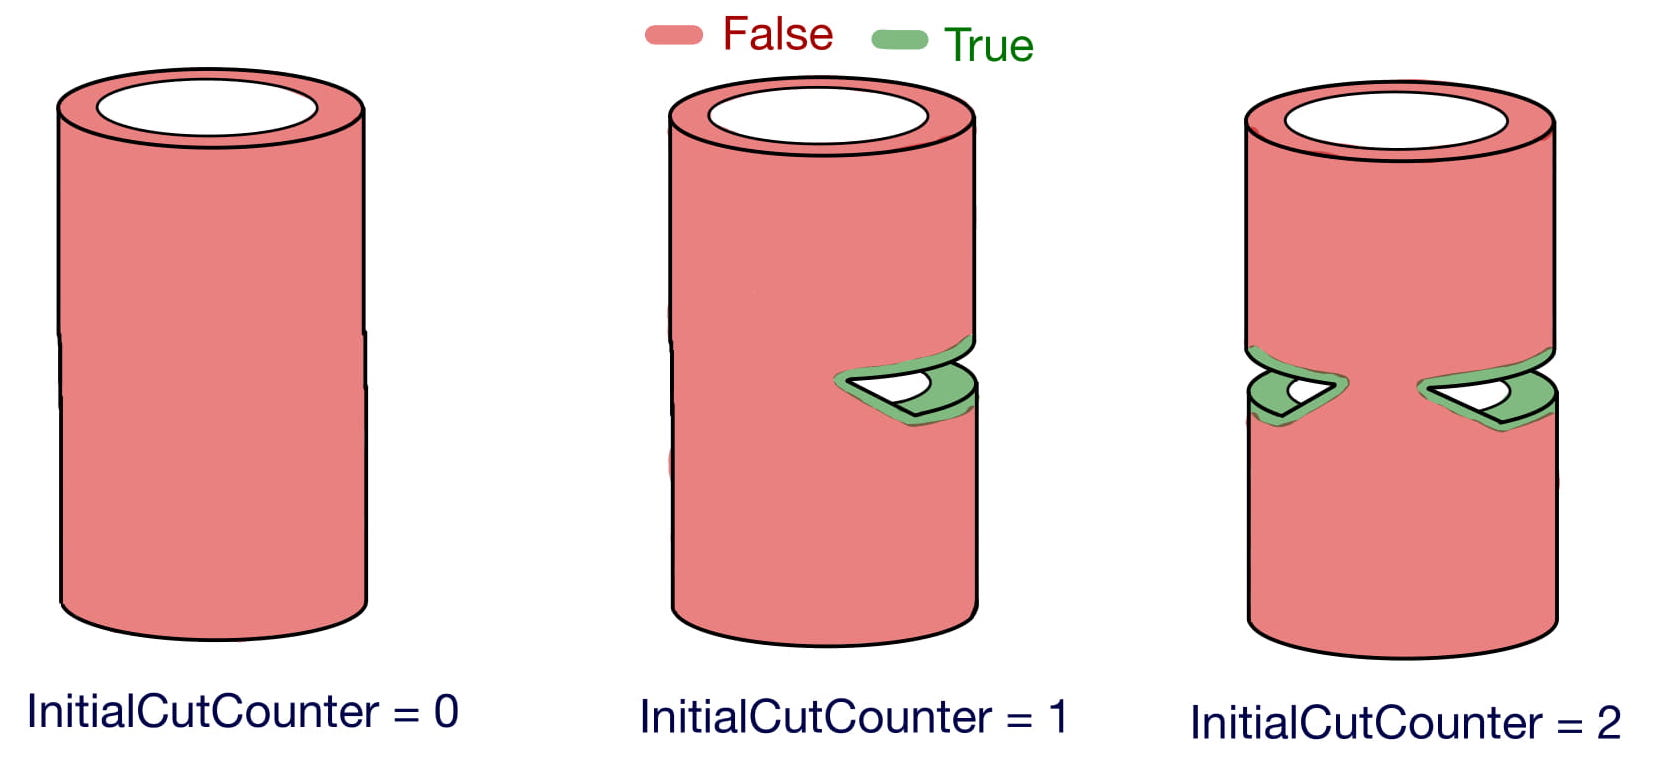
\includegraphics[width=1\textwidth]{validation/initial_cut.jpg}
  \caption{Counting the Number of Initial Cuts}
  \label{fig:ideal_cut}
\end{figure}


\paragraph{Unnecessary Collisions}
\label{para:data_counters_unnecessary_collisions}

An unnecessary collision is any collision between the tool and the mesh of interest made without a subsequent cut. This variable, $UnnecessaryCollisionsCounter$, counts the number of times the tool collided with the target mesh without the intention of performing a subsequent cut. The counter is incremented every time the user hits the rectal wall (the mesh behind the urethra) once the surgical tool touches an invisibile square.

\paragraph{Surgical Scene Exit}\label{para:data_surgical_scene_exit}

This variable, $SurgicalSceneExitCounter$, counts the number of times the tool exited the surgical scene.

\paragraph{Topological cuts}\label{para:data_counters_topological_cuts}

This variable, $topoligicalCutCount$, counts the number of topological cuts are on the urethra. One of the metrics that would allow for us to confirm whether the final resulting cut(s) from all the small snips ends up as a single cut is to see the number of disconnected cuts or holes there are in the mesh after the user completes the simulation. In an ideal end scenario, the resulting mesh would only have a single topological cut (ie, the mesh is seperated into two pieces without any other cuts in the two pieces). To calculate topological cuts, once a cut is performed, we take a set intersection between the triangles of the mesh after cutting and the initial mesh. The result of this would be the new triangles resulting from all cuts. By counting the number of disjoint group of triangles, we can identify the number of topological cut.

\subsubsection{Variables for Debugging}

\paragraph{Swipe Area of Blades}\label{para:data_swipe_area_of_blades}

\subparagraph{Case I: Single Blade}

This variable records the area swept by the blade from $t_1$ to $t_2$, where:

\begin{itemize}
  \item $t_1$: the initial collision between the tool and tube mesh
  \item $t_2$: the cut has been performed and the tool stops colliding with the mesh and starts moving away
\end{itemize}

An illustration is shown in Figure \ref{fig:single_blade_area}

\begin{figure}
  \centering%
  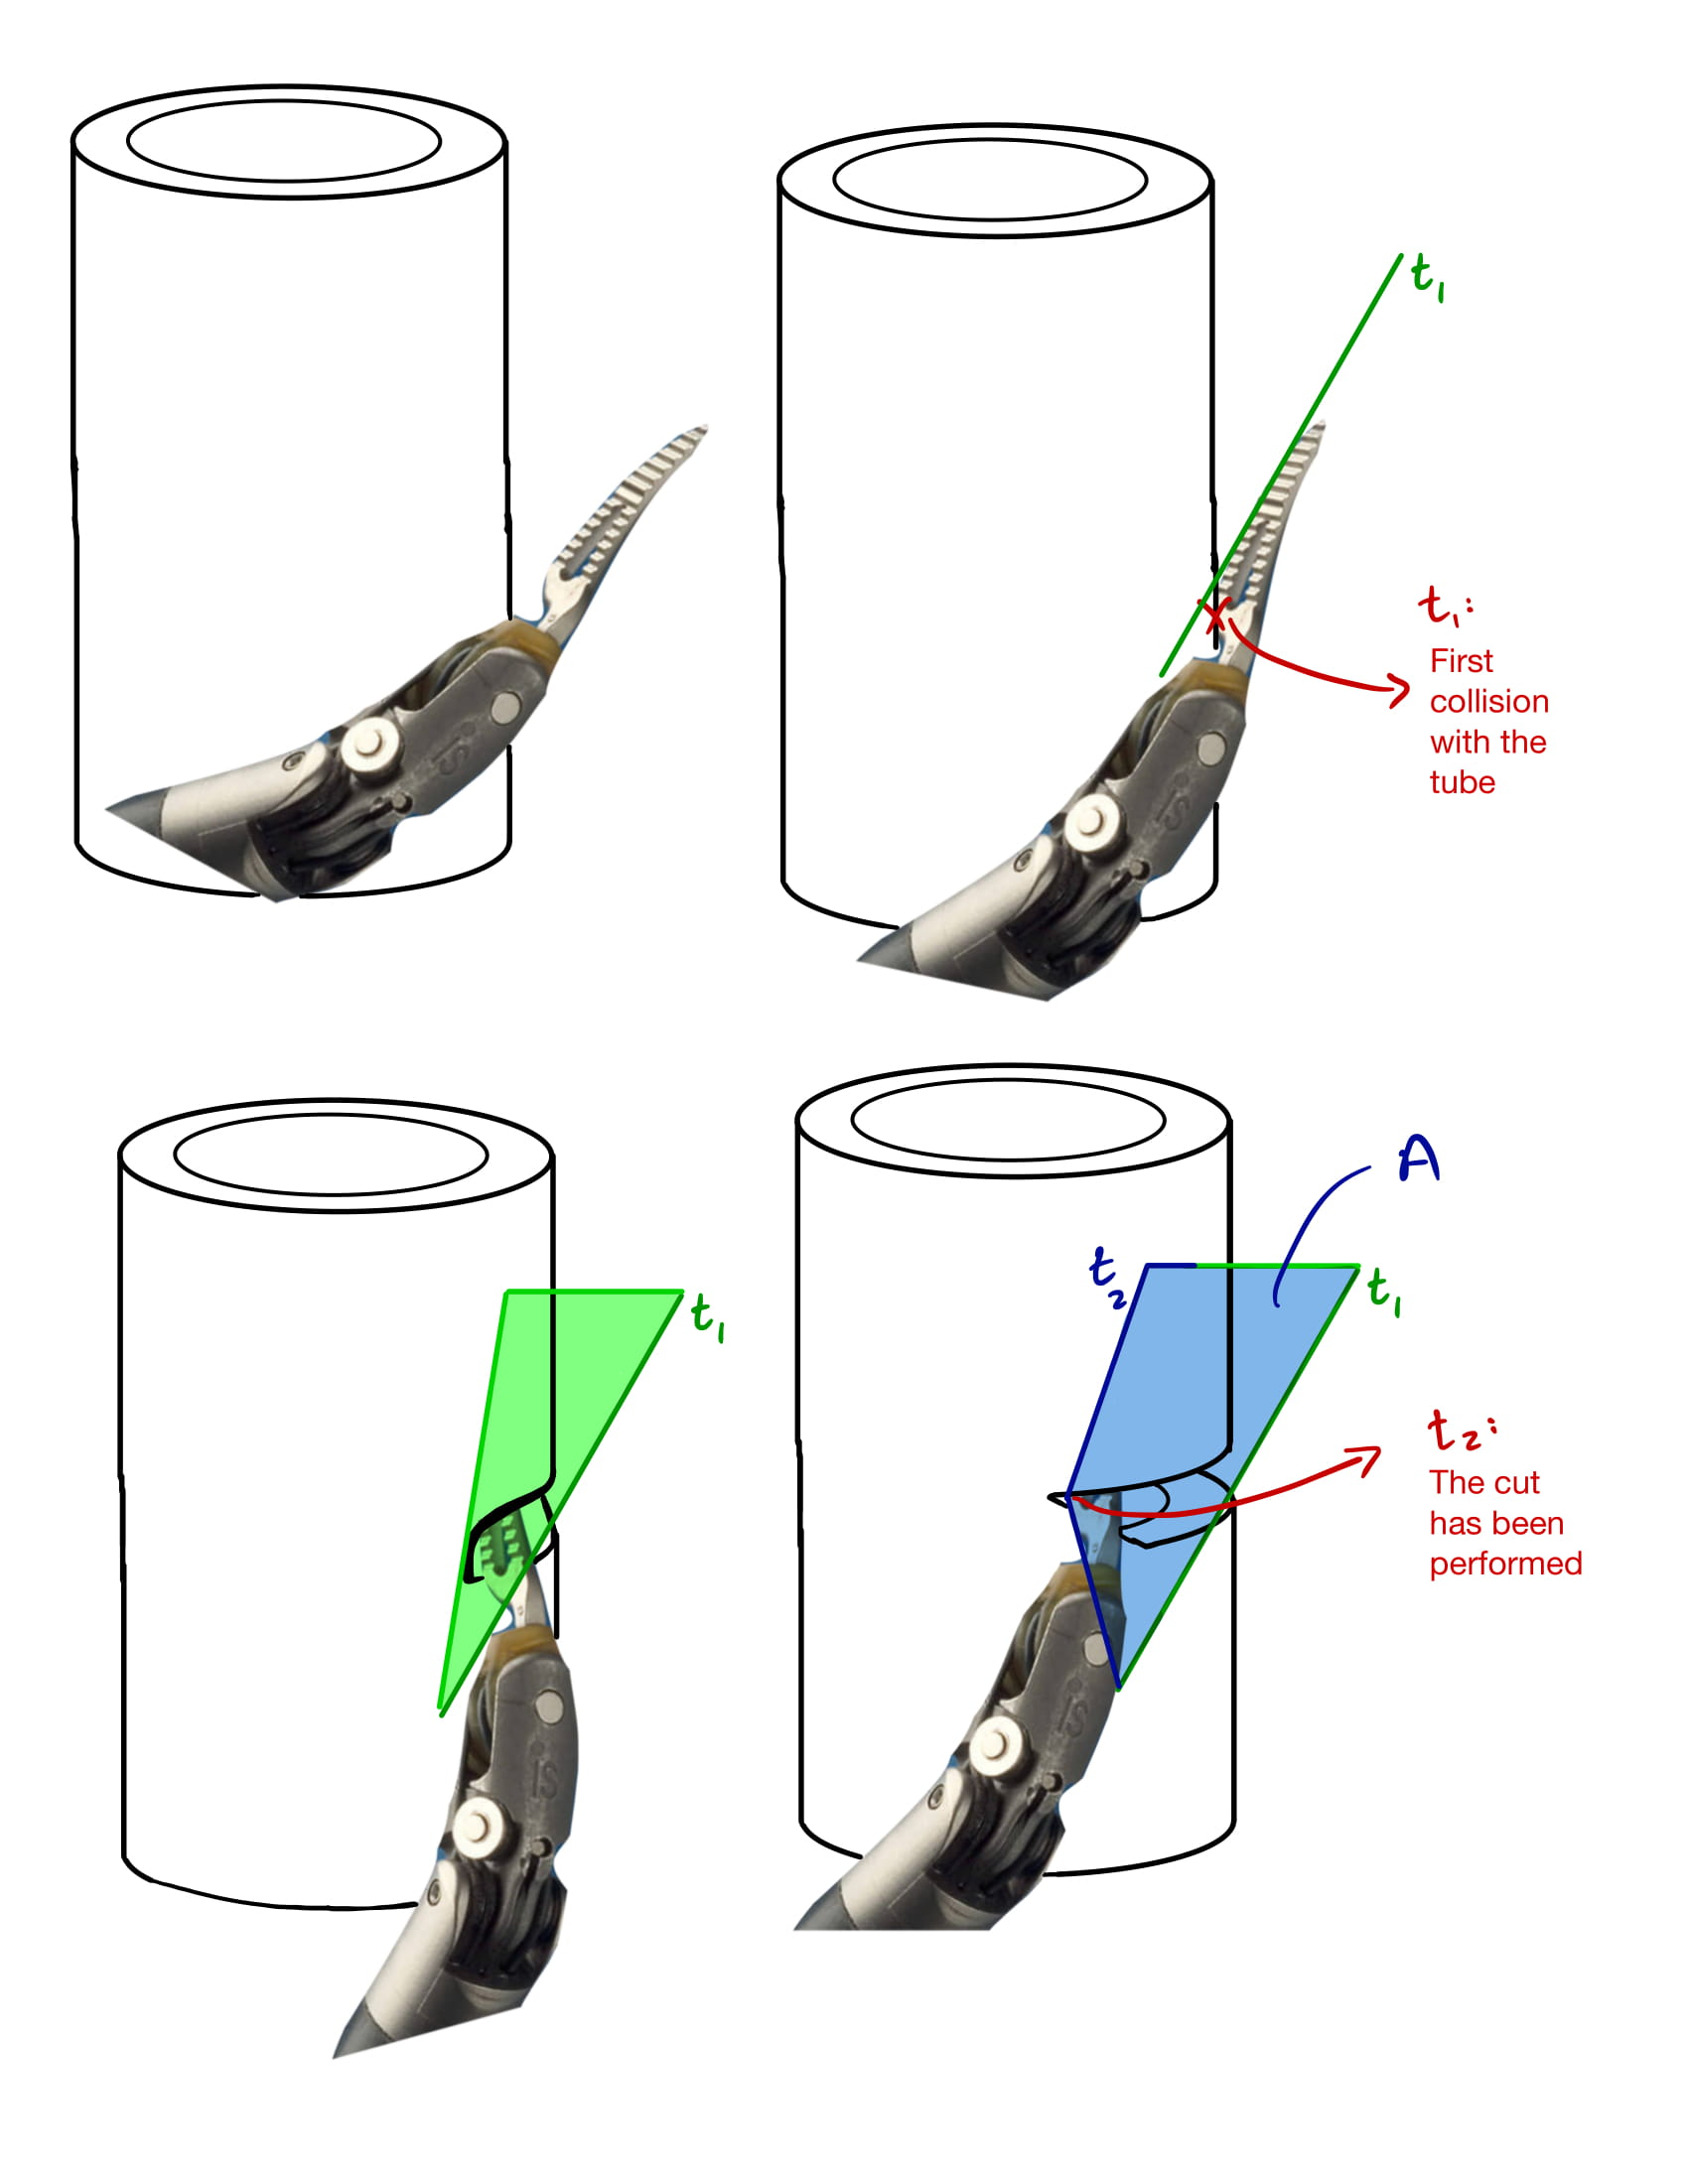
\includegraphics[width=0.7\textwidth]{validation/swipe_area_single_blade.jpg}
  \caption{Swipe Area Made by a Single Blade}\label{fig:single_blade_area}
\end{figure}

\subparagraph{Case II: Scissors}

This variable records the area swept by scissors upon performing a cut, as shown in Figure \ref{fig:scissors_area}.

\begin{figure}
  \centering%
  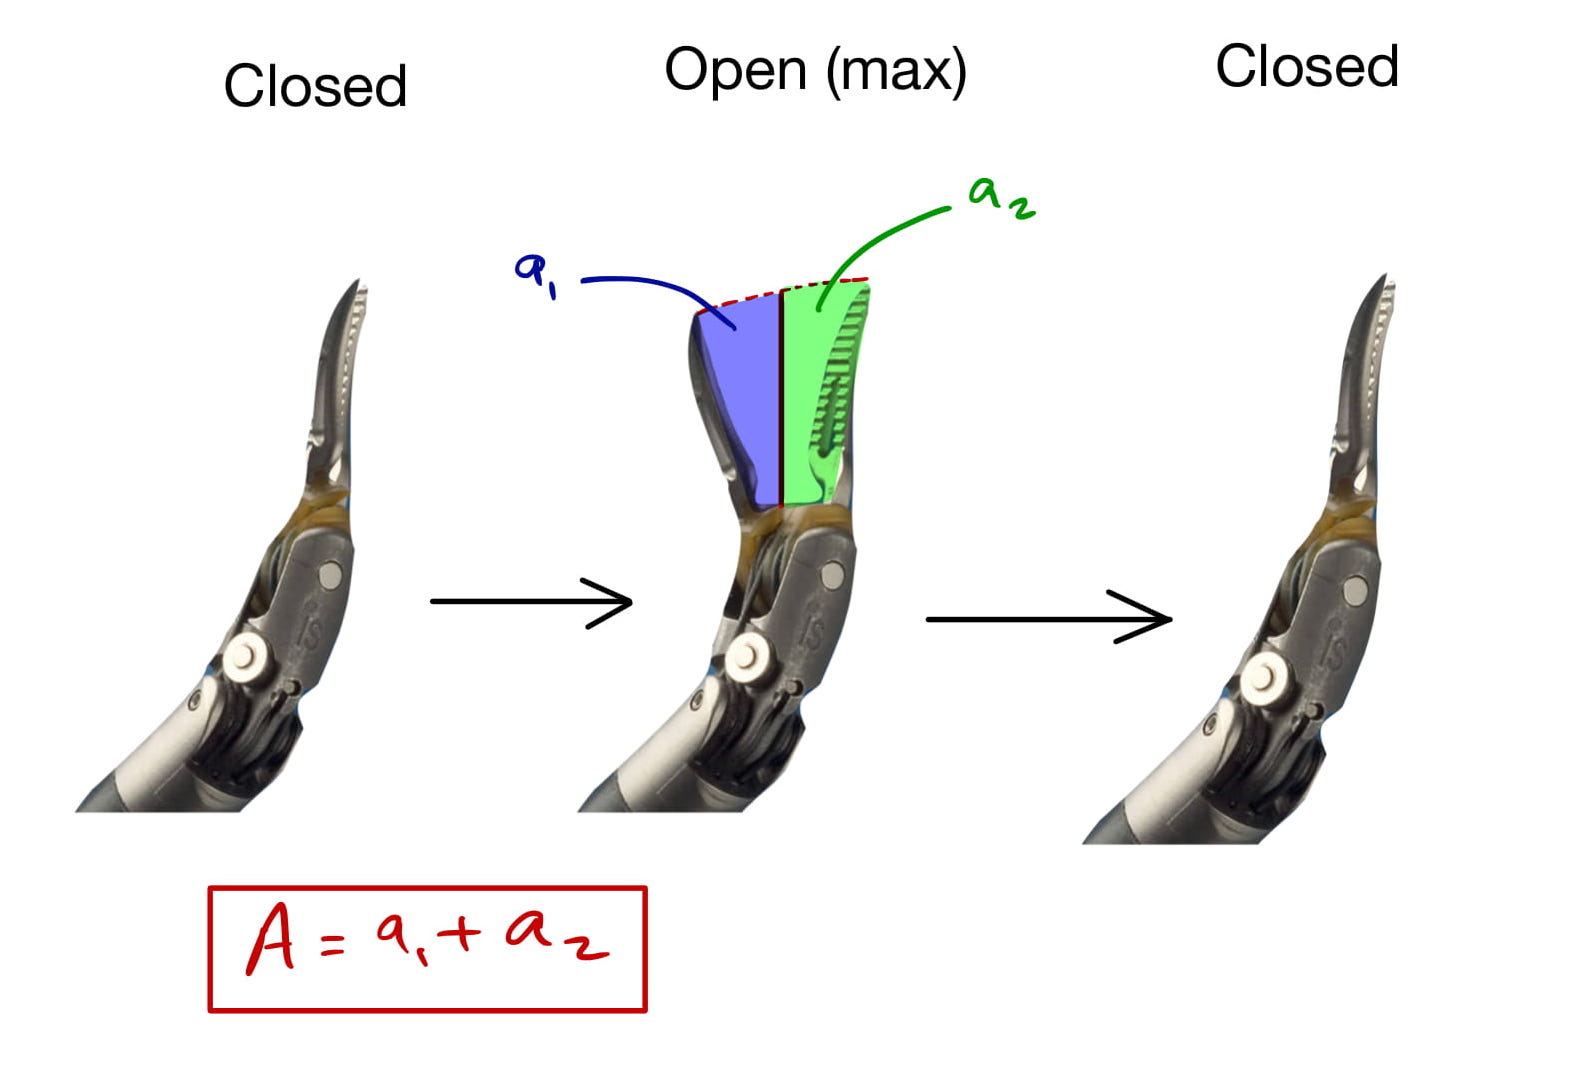
\includegraphics[width=0.7\textwidth]{validation/swipe_area_scissors.jpg}
  \caption{Swipe Area Made by Scissors}\label{fig:scissors_area}
\end{figure}

\subsubsection{Coordinates and Angle of Blades}\label{para:data_coordinates_of_blades}

The $4\times 4$ transformation matrix of the tooltip $\mathbf{M}(t)$. This will give both location and orientation. In case of scissors, an additional variable representing the angle of open and close state would be stored.


\subsection{Recording Metrics}\label{chp:literature}

\subsubsection{Complex metrics}
For recording metrics that have complicated structures required for the specified validations, we went for the serialization library that comes with Boost collection. The library allows for serializing C++ structs into boost format (written in ASCII). The serialized data can be de-serialized at a later stage and then converted into any format necessary for analysis and validation. A serialize function needs to be provided within structs that should be serialized. Boost serialization library provides a method to write serialization functions for data types that cannot be modified to include a serialize function such as with \texttt{glm} vectors, matrices that are required for recording metrics. The steps one should know are as follows:

\begin{enumerate}
    \item Non-intrusive serialization for library defined data types
    To serialize data types defined by libraries such as \texttt{glm} without modifying them, \texttt{boost::serialization} library provides a way to write serialization functions externally. For logging the required metrics, we use \texttt{glm} vectors, quaternions and matrices within structs created for logging. \autoref{code:custom_serialize} shows how serializing functions can be written in non-intrusively.
    \begin{lstlisting}[style=CStyle, caption={Serializing custom data types},label={code:custom_serialize}]
using glm::mat4;
using glm::quat;
using glm::vec3;
using glm::vec4;
namespace boost {
  namespace serialization {
    template < class Archive >
      void serialize(Archive & ar, vec3 & p,
        const unsigned int /* version */ ) {
        ar & p.x & p.y & p.z;
      }
    template < class Archive >
      void serialize(Archive & ar, vec4 & p,
        const unsigned int /* version */ ) {
        ar & p.x & p.y & p.z & p.w;
      }
    template < class Archive >
      void serialize(Archive & ar, mat4 & p,
        const unsigned int /* version */ ) {
        ar & p[0] & p[1] & p[2];
      }
    template < class Archive >
      void serialize(Archive & ar, quat & p,
        const unsigned int /* version */ ) {
        ar & p.w & p.x & p.y & p.z;
      }
  } // namespace serialization
} // namespace boost
    \end{lstlisting}
    \item Writing a struct for serialization (\autoref{code:serializable_struct})
    \begin{lstlisting}[style=CStyle, caption={A struct with serialize function written within it.},label={code:serializable_struct}]
struct my_struct {
  vec3 position;
  quat orientation;
  region_struct(vec3 position, quat orientation):
    position(position), orientation(orientation) {}
  private:
    friend class boost::serialization::access;
  template < class Archive >
    void serialize(Archive & ar,
      const unsigned int version) {
      ar & position & orientation;
    }
};
    \end{lstlisting}
    \item Serialize an object of struct `my\_struct` to a stream (\autoref{code:write_serialized})
    \begin{lstlisting}[style=CStyle, caption={Writing struct to a stream}, label={code:write_serialized}]
boost::archive::text_oarchive oa(stream);
oa << m;
    \end{lstlisting}
    \item De-serializing (\autoref{code:read_serialized})
    \begin{lstlisting}[style=CStyle, caption={Reading/De-serializing struct from a stream},label={code:read_serialized}]
boost::archive::text_iarchive ia(s);
ls::log_cut_struct m1;
ia >> m1;
    \end{lstlisting}
\end{enumerate}

\subsubsection{Simple metrics}
As for metrics that can be represented with one to few variables, we used the spdlog library combined with Boost format library for logging it as comma separated values to files. We chose to use this combination of libraries to log simple metrics as shown in \autoref{code:simple_logging} since they were already part of the project for producing logs for debug.

\begin{lstlisting}[style=CStyle, caption={Example of simple metrics logging},label={code:simple_logging}]
void Logger::log_collision_count(float col_count) {
collision_logger->info(str(boost::format("%f,%f") % get_elapsed() % col_count));
}
\end{lstlisting}

\subsubsection{Recording complex and simple metrics}
The types of data logged are classified into three categories, resulting in total of three log files to be generated for a cutting task. For each of the required categories, we have created structs that have the required member variables.

NOTE: The constructors and serialization functions have been omitted for legibility.

\begin{enumerate}
    \item Per Cut: After data recorded after a single cut is completed, in the case of scissors, a single cut is defined from when the scissors open ($t_1$) near a mesh to when the scissors close ($t_2$), resulting in mesh deformation. In the case of a single blade, a single cut is defined from when a blade collides with a mesh ($t_1$), to when it is moved away from the mesh ($t_2$), resulting in mesh deformation. A struct that represents these information is shown in \autoref{code:cut_deformation_struct}
    \begin{lstlisting}[style=CStyle, caption={Cut deformation struct}, label={code:cut_deformation_struct}]
struct region_struct {
  vec3 position;
  quat orientation;
  vec3 shape;
}
struct log_cut_deformation_struct {
  double time_elapsed;
  region_struct predef_top;
  region_struct predef_bot;
  region_struct postdef_top;
  region_struct postdef_bot;
  region_struct blade_swipe_region;
}
    \end{lstlisting}
    The variables recorded per cut includes top and bottom regions for pre deformation and post deformation. Additionally, we also record the time elapsed since beginning of simulation. To represent a region, we have created a nested struct that holds position, orientation and the vertices of the region.
    \begin{figure}
      \centering%
      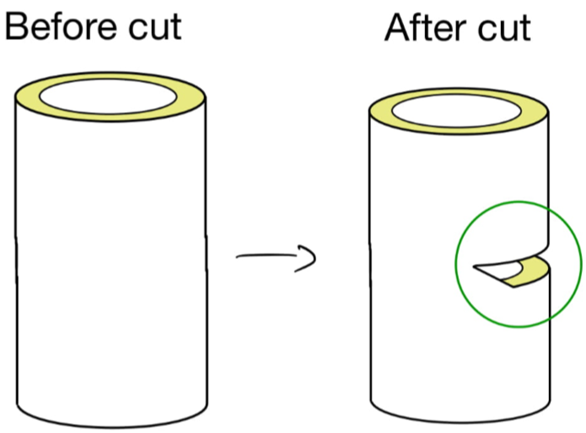
\includegraphics[width=0.7\textwidth]{validation/before_after_cut.png}
      \caption{Mesh change before and after cut}\label{fig:before_after_cut}
    \end{figure}

    \item Per Collision: Data recorded at each collision between the tool and the mesh of interest.\autoref{code:per_collision}
    \begin{lstlisting}[style=CStyle, caption={Log per collision}, label={code:per_collision}]
Logger::log_collision_count(float col_count) {
  collision_logger - > info(str(boost::format("%f,%f") % get_elapsed() %
    col_count));
}
    \end{lstlisting}
   Per collision, we record the time elapsed since start of simulation along with a counter that tracks unnecessary collisions. The data is stored as comma separated values, with each call to the function being written to a new line.

    \item Per Time Frame: Data recorded at all times. (\autoref{code:per_timeframe})
    \begin{lstlisting}[style=CStyle, caption={Struct for logging per time frame}, label={code:per_timeframe}]
struct log_per_time_frame_struct {
  double time_elapsed;
  mat4 blade_frame;
  int exit_counter;
}
    \end{lstlisting}
    During each time frame, we are recording the frame of the blade in represented by a 4x4 matrix, the time elapsed since start of simulation and an exit counter that counts the number of times the tool exited the surgical scene.

\end{enumerate}

% Commented part is to be deleted
% \subsection{Evaluation Protocols}\label{sec:evaluation}

% The validity tests we are performing at this stage of research are carried in a form of a formative usability study. A formative usability study is an iterative process of multiple usability testing approaches to evaluate the system being developed and assess the integration of features to ensure detecting and eliminating usability issues early before the final design is produced.

% Formative evaluation focuses on qualitative results collected from a variety of evaluators, including the design and development team, experts in the field, and target users. In the case of our simulation interface, participants in formative evaluations include the research team, expert surgeons, surgery training professionals, medical doctors with a background in prostatectomy, and surgeons-in-training. These methods are tailored to focus on the face, content and construct parameters of the simulator.

% The data collected from the described formative usability testing methods is primarily qualitative.  This data can be later categorized into areas of improvement and used to enhance the simulator for running the next iterations of formative evaluation tests. This qualitative data describes the state of each of the heuristics for face, content and construct validity and list usability issues to be resolved and areas of improvement.

% We are conducting two formative evaluation tests: heuristics evaluation and think-aloud evaluation, as described in following sub-sections.

% \subsubsection{Heuristics Evaluation}
% Heuristics evaluation is a formative evaluation method for finding the highest number of usability issues before the final design is produced. A list of heuristics is generated and tested through using the system of interest by a group of evaluators.

% \paragraph{Study Participants}
% The participants (or evaluators) in this method are not the target users, but usability experts and domain experts. A diverse group of evaluators ensures finding different types of and more usability issues. In the case of this project, this includes expert surgeons (whom this project is not targeted for, but can provide insights on the usability of the interface), the research team, and medical doctors with a background in prostatectomy.

% \paragraph{Study Structure}
% In heuristics evaluation, evaluators participate in two sessions: individual and group. In the individual session, the evaluator performs the cutting task and discusses a number of heuristics with the test moderator or the main usability researcher. In the group session, evaluators discuss their individual findings and propose solutions to these problems. The following is the detailed structure of each session.

% \subparagraph{Individual Evaluation Session} A session for where the evaluator individually completes and discusses the cutting task with the test moderator.
% \begin{enumerate}[1.]
%   \item Introduction (standardized with all evaluators):
%   \begin{enumerate}[\em a\em)]
%   \item Provide an overview of the project and the heuristics evaluation method,
%   \item Describe the current state and capabilities of the system,
%   \item Describe (and demo, if necessary) the cutting task.
%   \end{enumerate}
%   \item Allow the evaluator to freely use and explore the interface,
%   \item Guide the evaluator through the task, while discussing the heuristics,
%   \item Record the usability problems encountered or reported by the evaluator.
% \end{enumerate}

% \subparagraph{Group Debriefing Session}
% After individually testing with all the evaluators, organize a group meeting, list all the problems encountered with all evaluators, and discuss possible solutions.

% \paragraph{Cutting Task Heuristics}
% \begin{enumerate}[1.]
%   \item Face Validity:
% 	\begin{enumerate}[\em a\em)]
% 	  \item The cutting mechanism represents a real world cutting task in a prostatectomy surgery
% 	  \item The device is a sufficiently accurate representation of a real robotic system
% 	  \item The hand controllers are effective for working in the simulated environment
% 	  \item The user interface is efficient and minimalistic
% 	\end{enumerate}

%   \item Content Validity:
% 	\begin{enumerate}[\em a\em)]
% 	  \item The cutting task is effective for teaching the cutting skill for our target users
% 	  \item The scoring system effectively communicates the user's performance on the cutting exercise
% 	  \item The scoring system effectively guides the user to improve the performance on the simulator
% 	  \item The scoring system is effectively communicated to the user and messages are presented in plain language
% 	  \item Learning the system is feasible by first-time users with minimal supervision/training
% 	\end{enumerate}

%   \item Construct Validity:
% 	\begin{enumerate}[\em a\em)]
% 	  \item The system is able to distinguish between an experienced and a novice user based on errors
% 	  \begin{enumerate}[\em i\em)]
% 	    \item Number of times the cutting tool damages the tissue with unnecessary touches/cuts
% 	    \item Number of times the cutting tool goes outside the defined boundary
% 	  \end{enumerate}
% 	  \item The system is able to distinguish between an experienced and a novice user based on shape of cut
% 	  \begin{enumerate}[\em i\em)]
% 		  \item An interpolated plane of the overall cut (with a threshold for error tolerance)
% 		  \item The number of centimeters per small cut
% 		  \item The number of initial cuts
% 	  \end{enumerate}
% 	  \item The system is able to distinguish between an experienced and a novice user based on general statistics
% 	  \begin{enumerate}[\em i\em)]
% 		  \item Time taken to complete the test
% 	  \end{enumerate}
%   \end{enumerate}
% \end{enumerate}

% \subsubsection{Think-aloud Evaluation}
% Contrary to heuristics, the think-aloud method is performed with target users. In this method, the only data collected from the user is their thinking process throughout using the simulation and while completing the cutting task. Also, contrary to heuristics, the test moderator does not interfere or discuss the interface with the participant. Similar to heuristics, task completion is performed individually. This method is performed in three simple steps:

% \begin{enumerate}[1.]
%   \item Recruit representative subjects (target users)
%   \item Ask the subjects to complete the cutting task and describe their mental process as they complete the task
%   \item Meanwhile, the test moderator records the session and takes note of the interaction
% \end{enumerate}

% Following the session, the subjects filled a qualitative evaluation form including Likert-scale questions relating to face and content validity and discussed the interface informally with the team.

% \hrule%

% Based on the heuristic evaluation protocol, we prepared a questionnaire on a Likert Scale of 1 to 5, with 1 being \enquote{Strongly Disagree} to 5 being \enquote{Strongly Agree,} to validate and assess the simulator for face and content validity. The questions on Likert Scale will assist in assessing:
% \begin{enumerate}[\em i\em)]
%   \item The subjective realism of the simulator, \ie the face validity, and
%   \item Its appropriateness as a teaching modality, \ie the content validity.
% \end{enumerate}

% The questionnaire was provided to the evaluators after allowing them to freely use and interact with the cutting simulator. While using the cutting simulator, they were engaged in a discussion with the validity test moderator to assess the usability. Information about the participants (\emph{evaluators}) was collected. This enable classification of the feedback based on the experience level and specialization of the evaluator.

% Secondly, we have started implementation of the clinical metric for logging user interactions to assess construct validity. We have identified the information, described in Aim 5: Training and Test Scenarios, to be logged during the interaction of the evaluator with simulator. The information will be displayed after the completion of the task, as displayed in the graphical user interface described in Aim 5: Training and Test Scenarios.

% We have attached the following:
% \begin{enumerate}[1.]
%   \item A document used to collect information related to validation studies focusing on face and content validity (\autoref{apn:questionnaire}),
%   \item A summary of the scoring based on aforementioned questionnaire and feedback collected during the study (\autoref{apn:responses}), and
%   \item A report describing implementation of logging mechanism for construct validity (\autoref{apn:logging}).
% \end{enumerate}

% \hrule
% % TO BE DELETED
% Validation is an iterative assessment process throughout the prototype's development cycle to evaluate it from different perspectives: how it looks, how efficient it is, \etc.  We chose to conduct face, content, and construct validity to evaluate the simulator's realism, appropriateness as a teaching modality, and how good it is to differentiate between novice and expert surgeons, respectively.
% For this, we have developed a validation protocol, which we followed to conduct the studies. The protocol details are in the section below.

% \subsubsection{Validation Study Protocol}\label{sec:protocol}


% \paragraph{Pre-evaluation session}
% Estimated time: 10 minutes\\[-2ex]
% \hrule%
% The session moderator starts by taking permission for voice or video recording for future research use exclusively and letting them know that this session would take approximately one hour. Explaining the background of the surgical simulation with respect to urethral dissection and the technology under development. Moderator would use appropriate tools like a presentation and a RARP video. Using the think-aloud protocol, the surgeon is then asked to loudly express all their thoughts about the simulator, whether they are positive or negative. The surgeon is later asked to fill in a form with information such as name, speciality, number of experience years, and other relevant fields.

% \paragraph{Evaluation session}
% Estimated time: 30 minutes\\[-2ex]
% \hrule%
% During this session, the subject will manipulate a simulated model using the provided interface to get familiar with the setup at first. Then, the subject will start snipping the tubular structure (representing a urethra) and the user-interactions will be logged.
% While performing the snipping, the subject is expected to speak out their thoughts, while the moderator is asking them questions to get further feedback. The moderator shall remain unbiased while asking questions.
% A subject is expected to perform the same action (small snips on the urethra until it is completely detached in two pieces) five times.
% A unique identifier (ID) is assigned to each subject to preserve their anonymity. Since the procedure is repeated five times, the ID is assigned as follows, for instance: \texttt{50\_1}, \texttt{50\_2}, \texttt{50\_3}, \texttt{50\_4}, \texttt{50\_5}. \autoref{fig:subject} below shows the experimental setup during one of the evaluation studies:

% \begin{figure}
%   \centering
%   \includegraphics[width=.7\textwidth,frame]{validation/subject}
%   \caption{A urologist performing the cutting task}
%   \label{fig:subject}
% \end{figure}

% \paragraph{Post evaluation session}
% Estimated time: 20 minutes\\[-2ex]
% \hrule%
% Once the subject finishes all five trials, the moderator asks him to fill in some questions related to face and content validity. They are also free to express any further feedback that was not addressed through the questionnaire.


\clearpage%
